\documentclass[a4paper]{article}
\usepackage[margin=3.5cm]{geometry}
\usepackage{amsmath}
\usepackage{amssymb}
\usepackage[svgnames]{xcolor}
\usepackage{amsthm}
\makeatletter
\def\th@plain{%
  \thm@notefont{}% same as heading font
  \itshape % body font
}
\def\th@definition{%
  \thm@notefont{}% same as heading font
  \normalfont % body font
}
\makeatother
\usepackage{dsfont}
\usepackage{graphicx}
\usepackage{caption}
\usepackage{hyperref}
\usepackage{datetime}
\usepackage{outlines}
\usepackage{float}
\usepackage{booktabs}
\usepackage{enumitem}
\usepackage{mathtools}
\usepackage{nicematrix}
\usepackage{nccmath}
\usepackage{lipsum}
\usepackage[activate={true,nocompatibility},final,tracking=true,kerning=true,spacing=true,factor=500,stretch=15,shrink=15]{microtype}

\addtolength{\skip\footins}{2mm}

\definecolor{fgcolor}{rgb}{0.345, 0.345, 0.345}
\newcommand{\hlnum}[1]{\textcolor[rgb]{0.686,0.059,0.569}{#1}}%
\newcommand{\hlstr}[1]{\textcolor[rgb]{0.192,0.494,0.8}{#1}}%
\newcommand{\hlcom}[1]{\textcolor[rgb]{0.678,0.584,0.686}{\textit{#1}}}%
\newcommand{\hlopt}[1]{\textcolor[rgb]{0,0,0}{#1}}%
\newcommand{\hlstd}[1]{\textcolor[rgb]{0.345,0.345,0.345}{#1}}%
\newcommand{\hlkwa}[1]{\textcolor[rgb]{0.161,0.373,0.58}{\textbf{#1}}}%
\newcommand{\hlkwb}[1]{\textcolor[rgb]{0.69,0.353,0.396}{#1}}%
\newcommand{\hlkwc}[1]{\textcolor[rgb]{0.333,0.667,0.333}{#1}}%
\newcommand{\hlkwd}[1]{\textcolor[rgb]{0.737,0.353,0.396}{\textbf{#1}}}%
\let\hlipl\hlkwb

\usepackage{framed}
\makeatletter
\newenvironment{kframe}{%
 \def\at@end@of@kframe{}%
 \ifinner\ifhmode%
  \def\at@end@of@kframe{\end{minipage}}%
  \begin{minipage}{\columnwidth}%
 \fi\fi%
 \def\FrameCommand##1{\hskip\@totalleftmargin \hskip-\fboxsep
 \colorbox{shadecolor}{##1}\hskip-\fboxsep
     % There is no \\@totalrightmargin, so:
     \hskip-\linewidth \hskip-\@totalleftmargin \hskip\columnwidth}%
 \MakeFramed {\advance\hsize-\width
   \@totalleftmargin\z@ \linewidth\hsize
   \@setminipage}}%
 {\par\unskip\endMakeFramed%
 \at@end@of@kframe}
\makeatother

\definecolor{shadecolor}{rgb}{.97, .97, .97}
\definecolor{messagecolor}{rgb}{0, 0, 0}
\definecolor{warningcolor}{rgb}{1, 0, 1}
\definecolor{errorcolor}{rgb}{1, 0, 0}
\newenvironment{knitrout}{}{} % an empty environment to be redefined in TeX


% code highlighting
\usepackage{minted}
\usepackage{xpatch}
\newminted[cminted]{python}{fontsize=\small}
\xpretocmd{\cminted}{\RecustomVerbatimEnvironment{Verbatim}{BVerbatim}{}}{}{}

% link coloring
\hypersetup{
   colorlinks,
   linkcolor={red!90!black},
   citecolor={green!40!black},
   urlcolor={blue!60!black}
}

% concatenation symbol (c.f. ++ in Haskell)
\newcommand\mdoubleplus{\mathbin{+\mkern-10mu+}}

% end of proof symbol
\newcommand{\newmarkedtheorem}[1]{%
  \newenvironment{#1}
    {\pushQED{\qed}\csname inner@#1\endcsname}
    {\popQED\csname endinner@#1\endcsname}%
  \newtheorem{inner@#1}%
}
% \renewenvironment{proof}{{\noindent\bfseries Proof.}}{*something*}
%\let\oldproofname=\proofname
%\renewcommand{\proofname}{\rm\bf{\oldproofname}}


\theoremstyle{definition}
%\newtheorem{eg}{Example}[section]
\newmarkedtheorem{eg}{Example}[section]
\newtheorem{observation}{Observation}[section]
\newtheorem{remark}{Remark}
\theoremstyle{plain}
\newtheorem{define}{Definition\hspace{0.25em}\ignorespaces}
\newtheorem{proposition}{Proposition}
\newtheorem{lemma}{Lemma}
\newtheorem{corollary}{Corollary}
\newtheorem{theorem}{Theorem\hspace{0.25em}\ignorespaces}
\newtheorem{assump}{Assumption\hspace{0.25em}\ignorespaces}

\newdateformat{monthyeardate}{\monthname[\THEMONTH] \THEYEAR}

\author{Jeroen van Riel}
\date{\monthyeardate\today}
\title{Autonomous vehicle scheduling in networks}

\begin{document}

\maketitle

% \tableofcontents

\newcommand\halfopen[2]{\ensuremath{[#1,#2)}}
\newcommand\openhalf[2]{\ensuremath{(#1,#2]}}


\section{Platoons in tandem of two intersections}

\begin{figure}
  \centering
  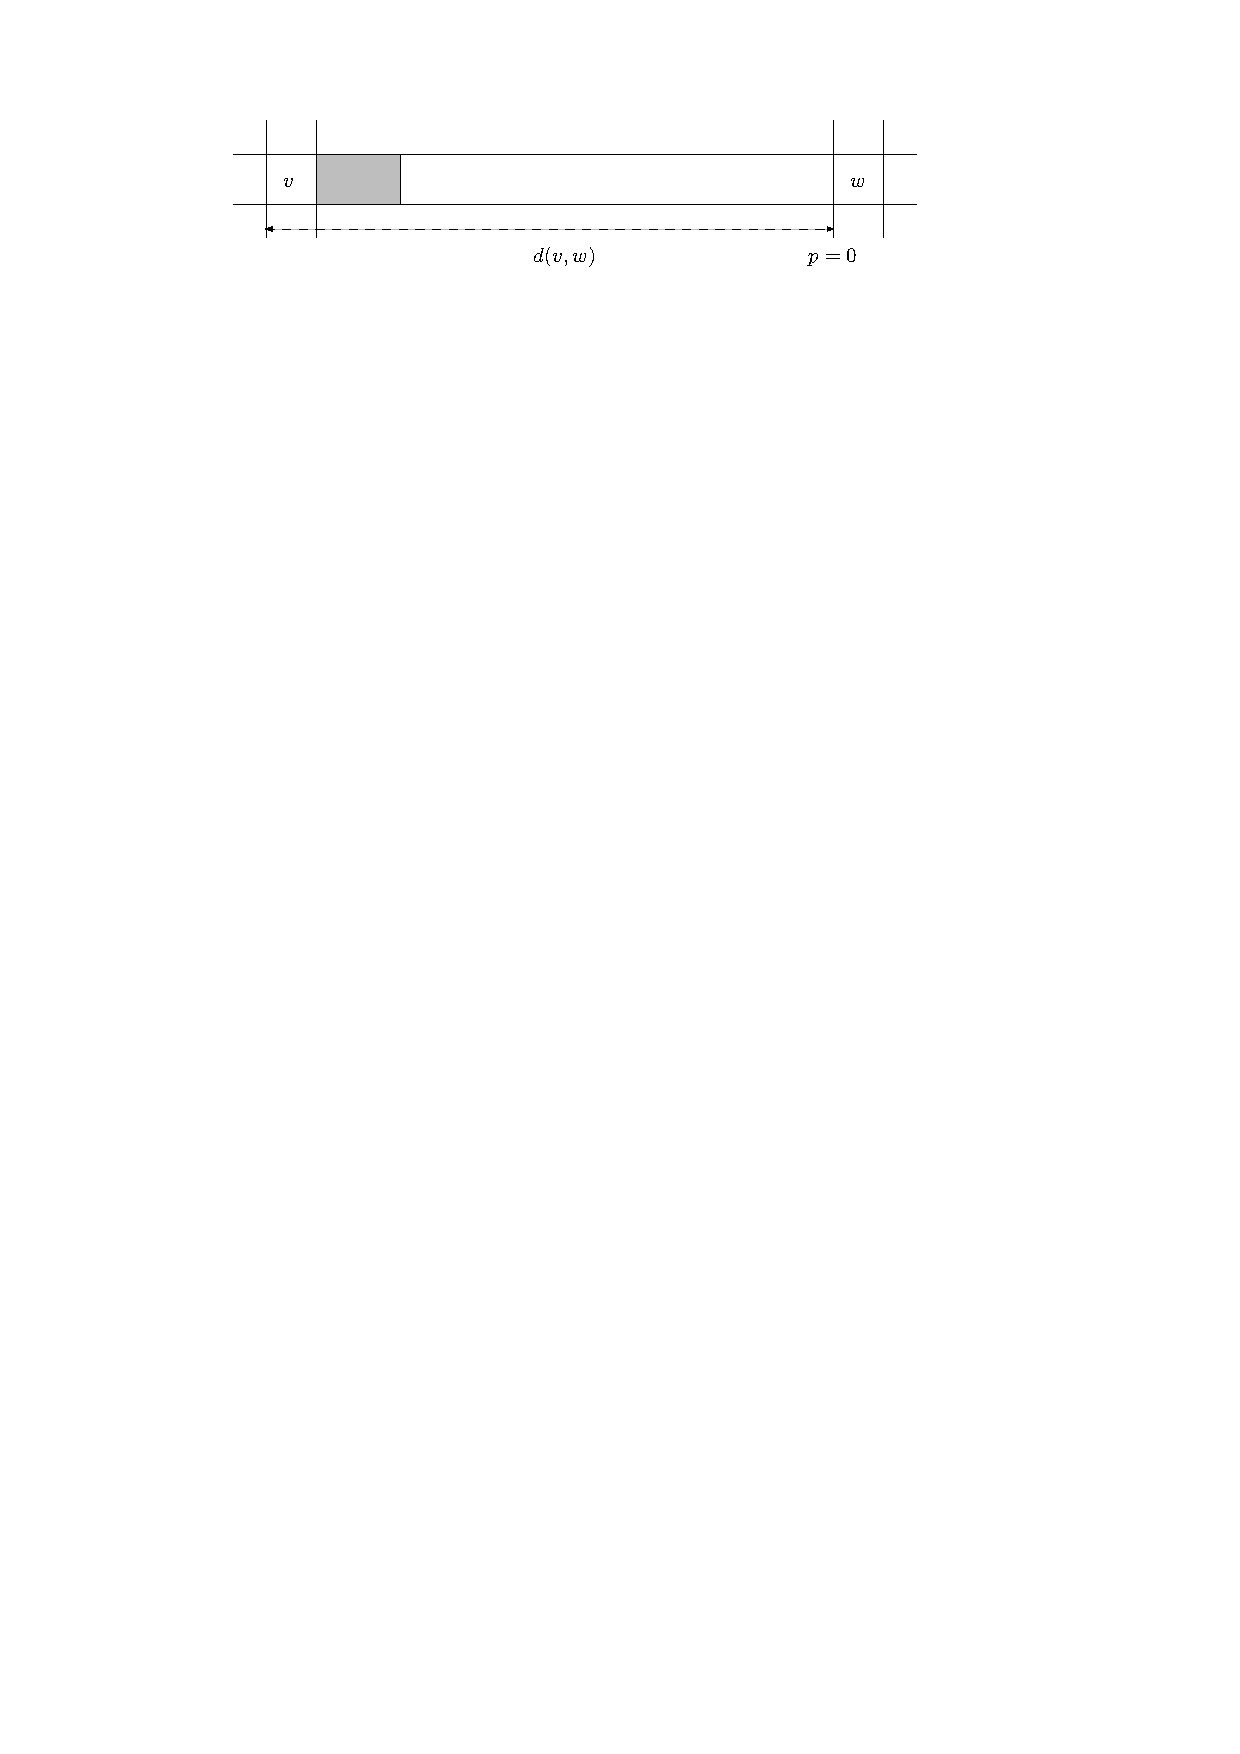
\includegraphics[width=0.99\textwidth]{figures/motion/tandem}
  \caption{Tandem of two intersections $v$ and $w$ with lane of length $d(v,w)$.
    The grey rectangle represents some vehicle that just left intersection $v$.
    We assume that vehicles must drive at maximum speed as long as they occupy
    any intersection, so deceleration is only allowed from the shown position
    onwards.}
  \label{fig:tandem}
\end{figure}

When considering multiple vehicles driving between intersection, we must take
into account the capacity of the lane segment between them, because the fact
that only a limited number of vehicles can drive or wait at the same time on a
lane between intersections may cause network-wide effects.
%
The capacity of lanes between intersections is intimately related to the
trajectories of vehicles, which we first want to understand better. We will be
using an optimal control formulation with the objective that keeps the vehicles
as close as possible to the next intersection at all times, which is similar to
the MotionSynthesize problem considered in
\cite{miculescuPollingsystemsbasedAutonomousVehicle2016}. This problem can be
solved using direct transcription, which works well enough if we just want to
simulate the behavior of the system. However, we show that it is possible to
explicitly formulate the optimal controller and explain how to compute
trajectories without using time discretization.

\subsection{Problem formulation}

Before we turn to the general case of networks of intersection, we will first
investigate the trajectories of vehicles in a tandem of two intersections as
depicted in Figure~\ref{fig:tandem}. Let $v$ denote the left intersection and
$w$ the right intersection and assume that vehicles drive from left to right.
% We will sometimes refer to intersection $w$ as the downstream intersection.
Furthermore, we will call the road segment strictly between both intersection
areas the \textit{lane}. In the following discussion, let $p(t)$ and $v(t)$ denote the
position and velocity of the vehicle, respectively, and we call
$x(t) = (p(t), v(t))$ its \textit{state}. Let the length and width of a vehicle
$i$ be denoted by $L_{i}$ and $W_{i}$, respectively. We measure the position of
a vehicle at the front bumper. We fix position $p=0$ at the stop line of
intersection $w$.
%
We make the following additional assumptions about our lane model.

\begin{assump}
  \label{assump:same_geometry}
  Vehicles are represented as rectangles, all having the same length $L_{i} = L$
  and width $W_{i} = W$. Lanes are axis-aligned and have width $W$, such that
  when lanes intersect, the intersection area is a square.
  Vehicles are not able to overtake other vehicle.
\end{assump}

\begin{assump}
  All vehicles satisfy the same double integrator dynamics
  $\dot{p} = v, \, \ddot{p} = u$ with velocity bounds
  $0 \leq v \leq v_{\max}$ and symmetric control
  bounds $-\omega \leq u \leq \omega$.
  We assume that the maximum
  speed is $v_{\max} = 1$, which is without loss of generality, because we can
  always achieve this by appropriate scaling of positions and the acceleration
  bound $\omega$.
\end{assump}

\begin{assump}
  \label{assump:full_speed}
  Vehicles drive at full speed when entering
  an intersection and keep driving at full speed as long as they occupy an
  intersection.
\end{assump}

Now assume that some vehicle is scheduled to start entering the lane at time
$t_{0} < 0$ and has to start entering $w$ at time $t=0$. Let
$p_{0} = -d(v,w) + W$ denote the position from where the vehicle starts to enter
the lane.
%
We will refer to the vehicle driving in front of the current vehicle as the
\emph{lead vehicle}. Let $\bar{p}(t)$ denote the position of rear bumper of the lead vehicle,
assuming there is one.
%
To avoid collision with this vehicle, the current vehicle must satisfy the \textit{lead}
constraint $p(t) \leq \bar{p}(t)$ at all times.
%
We try to keep the vehicle as close to $w$ as possible at all times. This yields
the optimal control problem
\begin{equation}
  \label{eq:optimal_control}
  \begin{aligned}
  \max_{u}    \quad & \int_{t_{0}}^{0} p(t) dt \\
    \begin{alignedat}{2}\text{s.t.}\\\\ {}\end{alignedat}
              \quad &\begin{alignedat}{2}
                     &\dot{p}=v, \; \ddot{p} = u , \\
                     &p(t_{0}) = p_{0} , \;\; &&  p(0) = 0 , \\
                     &v(t_{0}) = 1 ,  && v(0) = 1 , \\
                    \end{alignedat} \\
                    &\begin{alignedat}[t]{2}
                     {-\omega} \leq \; &u(t) \leq \omega , \\
                     0 \leq \; &v(t) \leq 1 , \\
                    \end{alignedat} \\
                    &\quad p(t) \leq \; \bar{p}(t) .
  \end{aligned}
\end{equation}


\subsection{Optimal control}

The aim of this section is to provide an explicit parameterization of optimal
solutions of problem~\eqref{eq:optimal_control}.
%
Before we proceed, we first rewrite it to the following standard form of optimal
control problems
\begin{align}
  \label{eq:standard_problem}
  \begin{split}
  \max \quad & \int_{t=t_{0}}^{t_{f}} F(x(t), u(t), t) dt \\
  \text{ s.t. } \;\, & \dot{x}(t) = f(x(t), u(t), t) , \quad x(t_{0}) = x_{0} , \\
             & a(x(t_{f}), t_{f}) \geq 0 , \\
             & b(x(t_{f}), t_{f}) = 0 , \\
                & g(x(t), u(t), t) \geq 0 , \\
             & h(x(t), t) \geq 0 ,
  \end{split}
\end{align}
where $x$ is the vector of state variables and $u$ is the control input.
%
Here, the constraints $g$ are called mixed state constraints, because they
involve both state and control variables, while constraints $h$ are called pure
state constraints.
%
In this subsection, we will write the state as $x = (x_{1}, x_{2})$ with
position $x_{1}$ and velocity $x_{2}$. The control function $u$ again
corresponds to acceleration. The initial state is $(p_{0}, v_{0})$ and the
target state is $(0, 1)$. We write $v_{0}$, because we will be considering
optimal trajectories with $v_{0} < 1$ as an intermediate step of the analysis.
%
Let $\bar{x}$ denote the state trajectory of the rear bumper of the lead vehicle.
%
With this new notation, optimal control problem~\eqref{eq:optimal_control} is equivalent to~\eqref{eq:standard_problem} for
$v_{0} = 1$ and setting\footnote{Instead of using quadratic expressions, constraints $g$ and $h_{1}$ could have each been written as two linear constraints, e.g., we could have chosen $g(x, u, t) = (\omega - u, \omega + u)$. However, this would violate the constraint qualification conditions of the theorem that we use in Section~\ref{sec:single_vehicle}.}
% \begin{align}
%   \label{eq:settings}
% \begin{split}
%   F(x, u, t) &= x_{1} , \\
%   f(x, u, t) &= (x_{2}, u) , \\
%   x_{0} &= (p_{0}, v_{0}) , \\
%   b(x, t) &= (x_{1}, x_{2} - 1) , \\
%   g(x, u, t) &= \omega^{2} - u^{2} , \\
%   h_{1}(x, t) &= x_{2} - x_{2}^{2} , \\
%   h_{2}(x, t) &= y_{1}(t) - x_{1} - L .
% \end{split}
% \end{align}
\[
\renewcommand{\arraystretch}{1.2}
\begin{NiceArray}{ r r @{} >{{}}c<{{}} @{} l l @{} }
  &t_{f} &=& 0 , \\
  &\;F(x, u, t) &=& x_{1} , \\
  &f(x, u, t) &=& (x_{2}, u) , \\
  (\text{2a}) \,\;\quad & x_{0} &=& (p_{0}, v_{0}) , & \Block{2-1}{\;\,(\text{2b})} \\
  &b(x, t) &=& (x_{1}, x_{2} - 1) , \;\; \\
  &g(x, u, t) &=& \omega^{2} - u^{2} , \\
  &h_{1}(x, t) &=& x_{2} - x_{2}^{2} , \\
  &h_{2}(x, t) &=& \bar{x}_{1}(t) - x_{1} . \;\,
\label{eq:setting}
\CodeAfter\SubMatrix.{1-1}{8-4}\}
\CodeAfter\SubMatrix\{{1-2}{7-1}.
\end{NiceArray}
\]
%
We refer to problem (\hyperref[eq:setting]{2a}) as the \emph{single vehicle
  variant}, because ignoring the lead constraint is equivalent to
considering a single vehicle in the system. For both problem variants, we will
denote an instance using the tuple $z = (t_{0}, p_{0}, v_{0})$.

In the upcoming analysis, we will encounter control functions that switch
between no acceleration, full deceleration and full acceleration, to which we
might refer as \emph{bang-off-bang} control. Furthermore, we will see that optimal
solutions have a particularly simple structure, illustrated in Figure~\ref{fig:tandem_trajectory}, to
which we refer as \emph{alternating control}. The following definition makes
this notion precise and introduces the notation that we use to completely
characterize optimal trajectories.

\begin{figure}
  \centering
  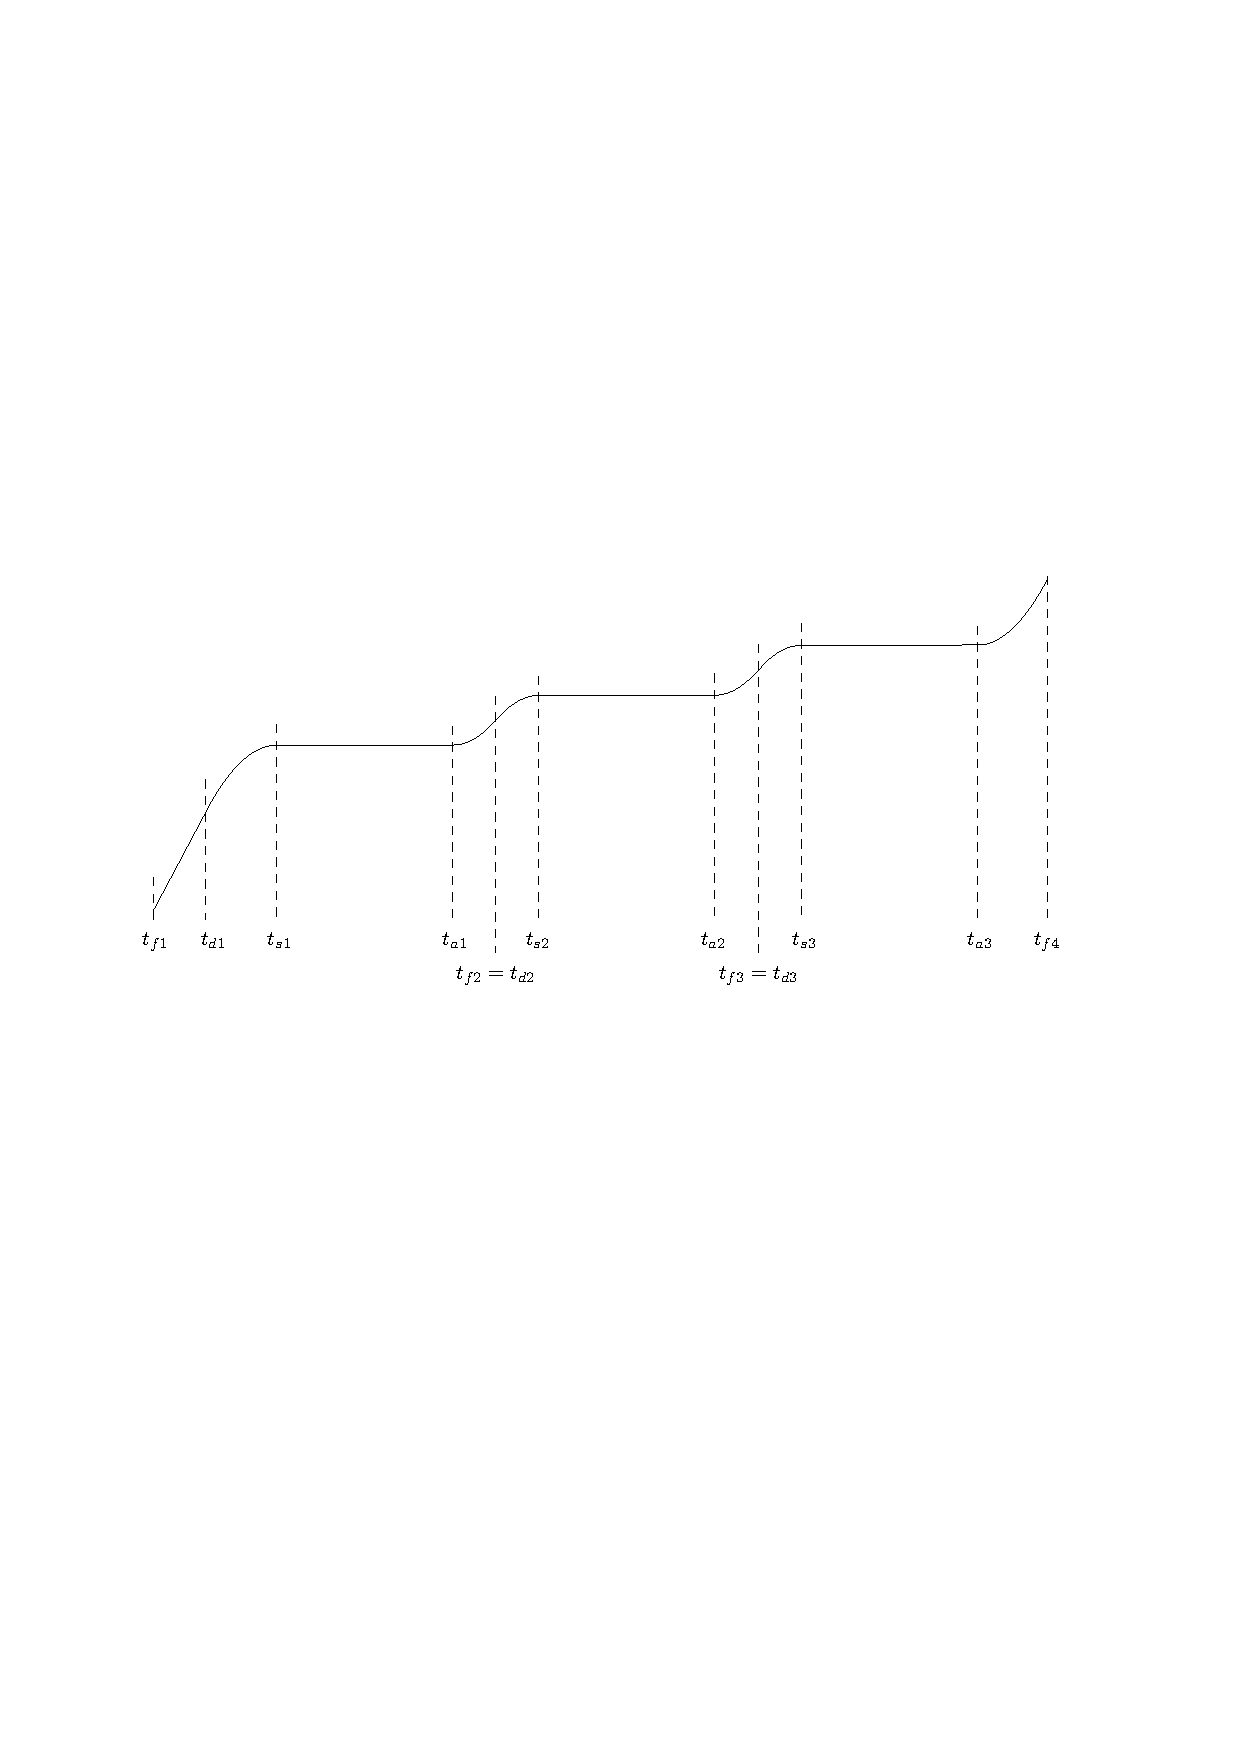
\includegraphics[width=0.99\textwidth]{figures/motion/tandem_trajectory}
  \caption{Some example of an alternating vehicle trajectory $x$. The particular
    shape of this trajectory is due to two preceding vehicles, which causes the
    two ``bumps'' at the times where these vehicles exit the lane. The
    trajectory of the current lead vehicle and previous lead vehicles that gave
    rise to this particular shape are not shown for clarity.}
  \label{fig:tandem_trajectory}
\end{figure}


\subsection{Feasibility of crossing times}

We now investigate the limit on the number of vehicles that can occupy the lane
when waiting. Imagine that vehicles enter the lane until it is full and then
only after all vehicles have come to a full stop, they start to leave the lane
by crossing $w$. We refer to the maximum number of vehicles that can wait in the
lane as the \textit{stationary lane capacity}.
%
Suppose that we want to design the tandem network that has a stationary lane
capacity of at least $c(v,w)$. Vehicles are required to drive at full speed as
long as they occupy any intersection. Therefore, a vehicle crossing $v$ can only
start decelerating after $p(t) \geq p_{0} + L$, so the earliest position where a
vehicle can come to a stop is $p_{0} + L + p^{+}(d_{f})$.
%
Because vehicles need to gain maximum speed before reaching $w$,
the position closest to $w$ where a vehicle can wait is $- p^{+}(d_{f})$.
%
Hence, in order to accomodate for $c(v,w)$ waiting vehicles, the length of the
lane must satisfy
\begin{align*}
  d(v, w) \geq W + L + 2p^{+}(d_{f}) + (c(v,w) - 1) L ,
\end{align*}
as illustrated in Figure~\ref{fig:tandem_annotated}.
%
Conversely, given the lane length $d(v,w)$, the corresponding stationary lane
capacity is given by\footnote{Without Assumption~\ref{assump:same_geometry}, we
  cannot derive such a simple formula, because it would depend on the specific
  lengths of those vehicles currently in the system.}
\begin{align*}
  c(v, w) = \texttt{floor}\left( \frac{d(v,w) - W - 2 p^{+}(d_{f})}{L} \right) ,
\end{align*}
where $\texttt{floor}(x)$ denotes the largest integer smaller than or equal to
$x$.

{\color{Navy}
% emphasize fixed locations
It turns out that the fixed locations where vehicles wait in the above scenario
are helpful in describing the optimal trajectories, even when vehicles never
fully stop. We will denote these fixed \textit{waiting positions} as
\begin{align*}
  p_{k} = - p^{*}(d_{f}) - (c(v,w) - k) L,
\end{align*}
for $k = 1, \dots, c(v,w)$.
%
Furthermore, let $p_{d} = p_{1} - p^{*}(d_{f})$ denote the position from
which vehicles must decelerate in order to stop at the first waiting position
$p_{1}$.
%
Now consider a vehicle that moves from $p_{k}$ to the next waiting position
$p_{k+1}$, so it moves exactly distance $L$. We consider such a start-stop
movement, without considering any safe following constraints. By symmetry of the
control constraints, the vehicle moves the same distance during both
acceleration and deceleration. Furthermore, the vehicle needs to be at rest at
the start and end of such trajectory. Hence, it is clear that it takes the same
amount of time $d_{s}$ to accelerate and decelerate. We assume that
$d_{s} < d_{f}$, which ensures that maximum velocity is never reached during the
start-stop movement, which is illustrated in Figure~\ref{fig:start-stop}. In this case, it is
clear that we must have $L = 2 p^{*}(d_{s})$, from which we derive that
$d_{s} = \sqrt{L / a_{\max}}$.
}


% \begin{figure}
%   \centering
%   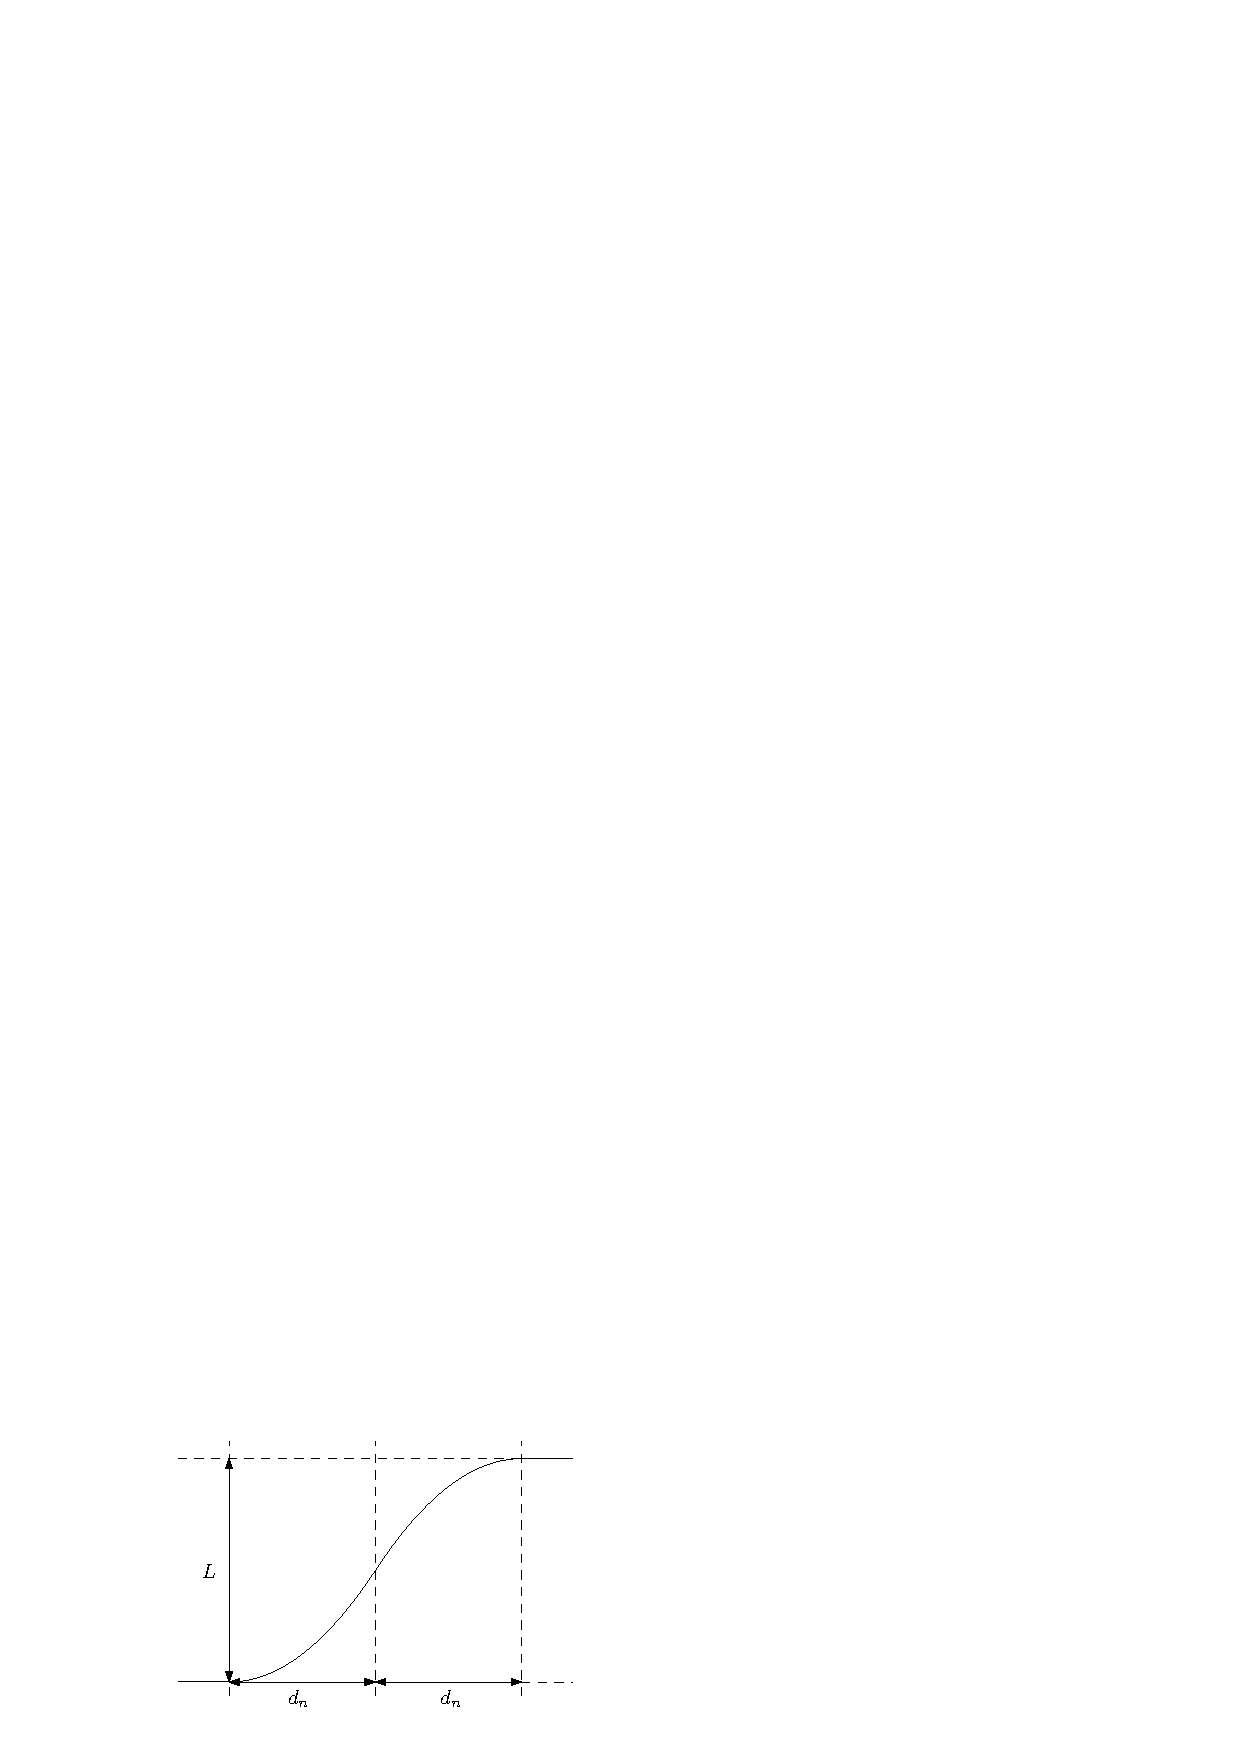
\includegraphics[scale=1.0]{figures/motion/start_stop_trajectory}
%   \caption{Shape of some start-stop trajectory of a single isolate vehicle
%     moving forward from some current waiting position $p_{k}$ to the next
%     $p_{k+1}$.}
%   \label{fig:start-stop}
% \end{figure}

% \begin{figure}
%   \centering
%   \includegraphics[width=0.99\textwidth]{figures/motion/merge}
%   \caption{Sketch how the initial deceleration merges with the first start-stop phase.}
%   \label{fig:merge}
% \end{figure}



% Finally, to simplify the upcoming analysis of optimal trajectories, we make the
% following assumption on lanes.

% \begin{assump}
%   Each lane has at least capacity for a single vehicle, so $c(v, w) \geq 1$,
%   or equivalently, the length of the lane must be at least
%   $d(v, w) \geq 2p^{+}(d_{f}) + W + L$, or in terms of the control problem
%   parameter $p_{0} \leq -2p^{+}(d_{f}) - L$.
% \end{assump}


\begin{figure}
  \centering
  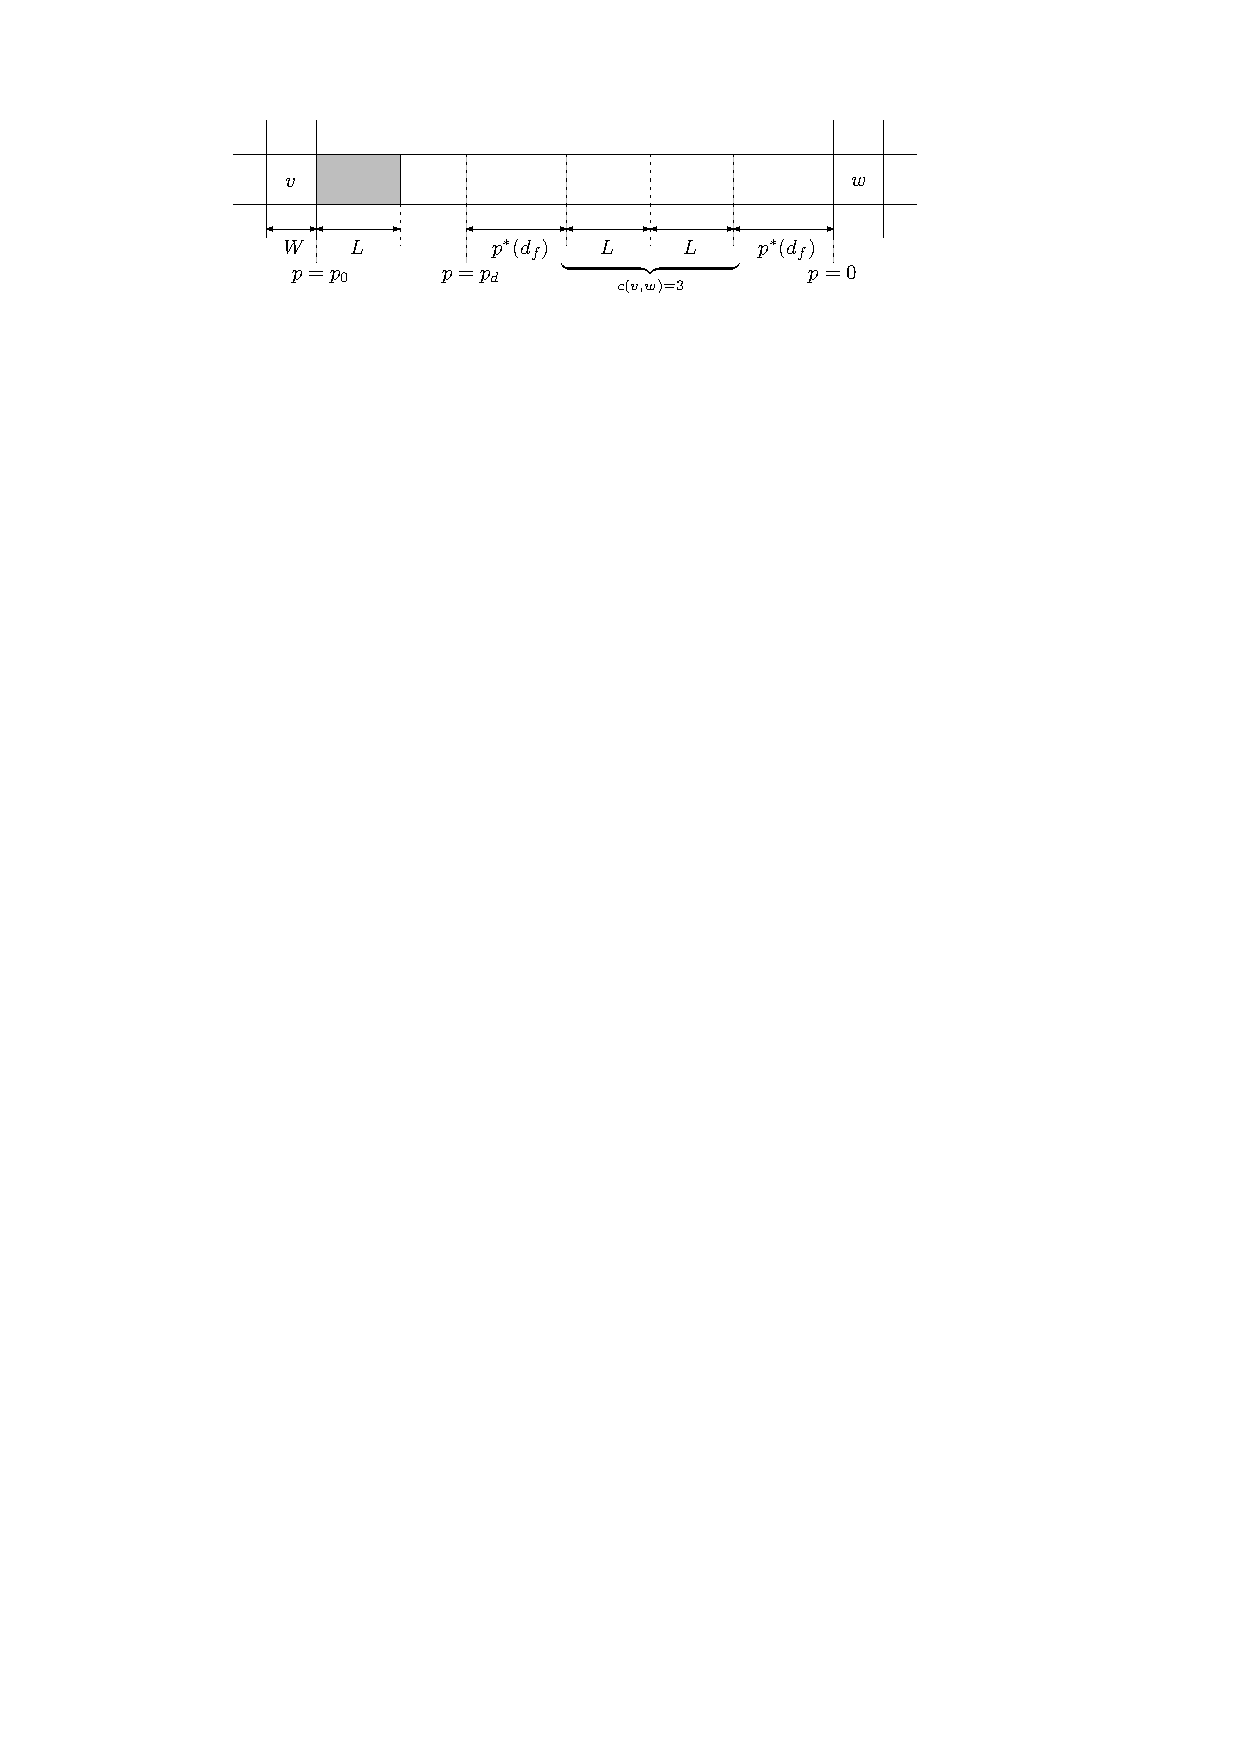
\includegraphics[width=0.99\textwidth]{figures/motion/tandem_annotated}
  \caption{Tandem of intersections with indicated distances used in the
    derivation of the stationary lane capacity, which is the maximum number of
    vehicles that can stop and wait in the lane, before they leave.}
  \label{fig:tandem_annotated}
\end{figure}


\newpage

\section{Vehicle scheduling in networks}

\begin{figure}
  \centering
  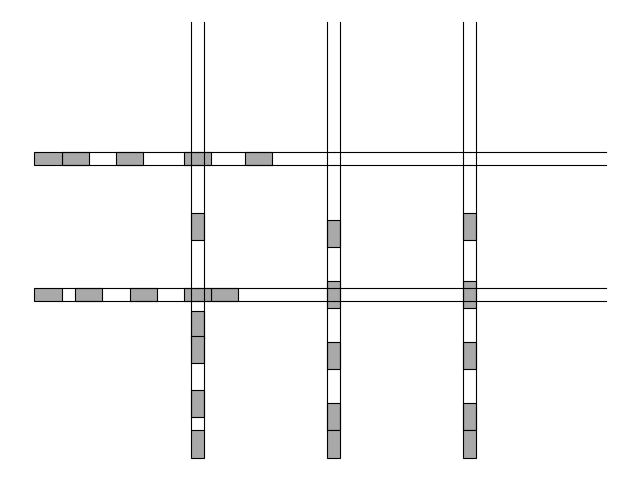
\includegraphics[width=0.55\textwidth]{figures/network/grid_example.png}
  \caption{Illustration of some grid-like network of intersections with vehicles
    drawn as grey rectangles. There are five vehicle routes: two from east to
    west and three from south to north. Turning at intersections is not
    allowed.}\label{fig:network_illustration}
\end{figure}

We now extend the single intersection model to a network of intersections
without turning routes, illustrated in Figure~\ref{fig:network_illustration}.
% network definition
We define a directed graph $(\bar{V},E)$ with nodes $\bar{V}$ and arcs $E$,
representing the possible paths that vehicles can follow. Nodes with only
outgoing arcs are \textit{entrypoints} and nodes with only incoming arcs are \textit{exitpoints}.
Let $V$ be the set of \textit{intersections}, which are all the nodes with
in-degree at least two.
%
Let $d(v, w)$ denote the distance between nodes $v$ and $w$.
%
For each route index $r \in \mathcal{R}$, we let
\begin{align*}
  \bar{V}_{r} = (v_{r}(0), v_{r}(1), \dots, v_{r}(m_{r}), v_{r}(m_{r}+1))
\end{align*}
be the path that vehicles $i \in \mathcal{N}_{r}$ follow through the network. We
require that the first node $v_{r}(0)$ is an entrypoint and that the last node
$v_{r}(m_{r}+1)$ is an exitpoint and we write
\begin{align*}
  V_{r} = \bar{V}_{r} \setminus \{ v_{r}(0), \, v_{r}(m_{r}+1) \}
\end{align*}
to denote the path restricted to intersections. We say that some $(v, w) \in E$
is on path $V_{r}$ whenever $v$ and $w$ are two consecutive nodes on the path
and we write $E_{r}$ to denote the set of all these edges. We require that
routes can only overlap at nodes by making the following assumption.

\begin{assump}\label{assump:disjoint_routes}
  Every arc $(v,w) \in E$ is part of at most one route $V_{r}$, such that routes
  do not share lanes. This ensures that the order of vehicles on each lane is
  completely determined by the order of vehicles on the corresponding lane.
\end{assump}

We start by considering networks in which all roads are axis-aligned such that
intersections always involve perpendicular lanes and where routes are such that
no turning is required. For each $v \in V_{r}$ define the conflict zone
$\mathcal{E}_{r}(v) = (b_{r}(v), e_{r}(v))$ and consider the union
\begin{align*}
  \mathcal{E}_{r} = \bigcup_{v \in V_{r}} \mathcal{E}_{r}(v)
\end{align*}
corresponding to the positions of vehicles $i \in \mathcal{N}_{r}$ for which it
occupies an intersection on its path $V_{r}$.
%
By reading $\mathcal{E}_{i} \equiv \mathcal{E}_{r}$ for $r(i) = r$, the single
intersection problem naturally extends to the network case. Like before, the
resulting problem can be numerically solved by a direct transcription method.

\begin{figure}
  \centering
  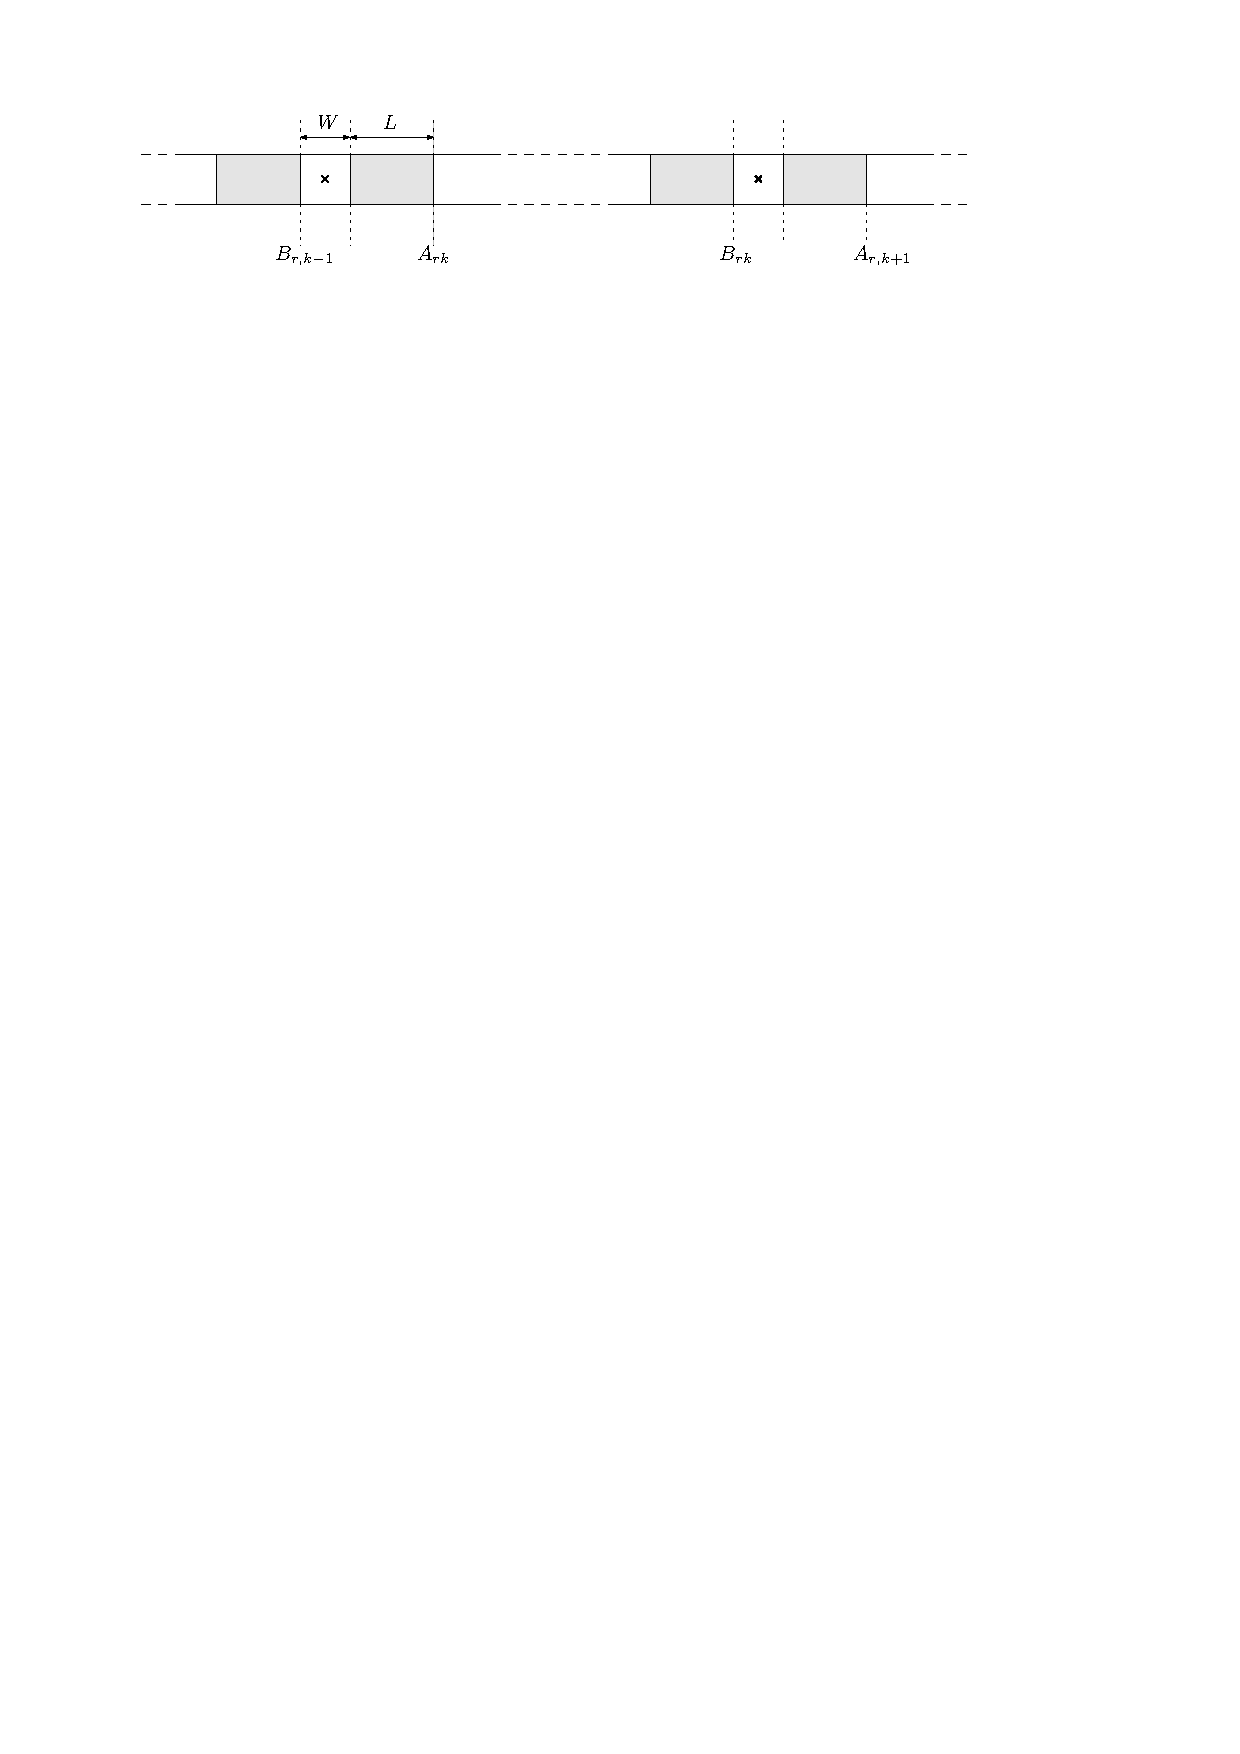
\includegraphics[scale=1]{figures/motion/intersection}
  \caption{Illustration of how the individual lane models are connected to form
    a route and how to model an intersection. The intersection region is marked
    with a little cross. The width of the vehicle $W$ is used as the length of
    the intersection. The longitudinal positions $A_{ij}$ and $B_{ij}$ denote
    the start and end, respectively, of the $j$th lane on route $i$.}%
  \label{fig:intersection}
\end{figure}

\subsection{General decomposition}
The general two-stage decomposition for the single intersection extends rather
naturally to the present model. Let for each pair $(i,v)$ of some vehicle
$i \in \mathcal{N}$ and an intersection $v \in V_{r(i)}$ along its route, let
\begin{align*}
\inf \{ t: x_{i}(t) \in \mathcal{E}_{r}(v) \} \;\; \text{ and } \; \sup \{ t: x_{i}(t) \in \mathcal{E}_{r}(v) \}
\end{align*}
be the crossing time and exit time, which we denote by $y(i,v)$ and
$y(i,v) + \sigma(i, v)$, respectively.
%
Instead of a single set of conflicts, we now define for each intersection
$v \in V$ in the network the set of conflict pairs
\begin{align*}
\mathcal{D}^{v} = \{ \{i,j\} \subset \mathcal{N} : r(i) \neq r(j), v \in V_{r(i)} \cap V_{r(j)} \} .
\end{align*}
Now the two-stage approach is to solve
\begin{align*}
  \min_{y,\sigma} \;\; & \sum_{r \in \mathcal{R}} F(y_{r}, \sigma_{r}) \\
  \text{ s.t. } & y(i,v) + \sigma(i,v) \leq y(j,v) \text{ or }  \\
                & y(j,v) + \sigma(j,v) \leq y(i,v) , & \text{ for all } \{i,j\} \in \mathcal{D}^{v} \text{ and } v \in V, \\
  & (y_{r}, \sigma_{r}) \in \mathcal{S}_{r} , \quad & \text{ for all } r \in \mathcal{R} ,
\end{align*}
%
where $F(y_{r}, \sigma_{r})$ and $\mathcal{S}_{r}$ are the value function and
set of feasible parameters, respectively, of the parametric trajectory
optimization problems
%
\begin{align*}
  F(y_{r}, \sigma_{r}) = \min_{x_{r}} & \; \sum_{i \in \mathcal{N}_{r}} J(x_{i}) \\
  \text{ s.t. } & x_{i}(t) \in D_{i}(s_{i,0}) , \quad & \text{ for } i \in \mathcal{N}_{r} , \\
  & x_{i}(y(i,v)) = b_{r}(v) , \quad & \text{ for } v \in V_{r} , i \in \mathcal{N}_{r} , \\
  & x_{i}(y(i,v) + \sigma(i,v)) = e_{r}(v) , \quad & \text{ for } v \in V_{r} , i \in \mathcal{N}_{r} , \\
  & x_{i}(t) - x_{j}(t) \geq L , \quad & \text{ for } (i, j) \in \mathcal{C} \cap \mathcal{N}_{r} ,
\end{align*}
where we again use subscript $r$ to group variables according to their associated route.


\subsection{Decomposition for delay objective}

Suppose we use use the crossing at the last intersection as performance measure, by defining the
objective function as
\begin{align*}
  J(x_{i}) = \inf \{ t: x_{i}(t) \in \mathcal{E}_{r}(v_{r}(m_{r}))\} .
\end{align*}
%
We show how to reduce the resulting problem to a scheduling problem, like we did
in the single intersection case.
%
We will again assume Assumption~\ref{assump:same_geometry} and
Assumption~\ref{assump:full_speed}, so vehicles will always cross intersections
at full speed, and all vehicles share the same geometry. Hence, the occupation
time $\sigma \equiv \sigma(i,v)$ is the same for all vehicles and intersections. For this
reason, we will write the shorthand $y_{r} \in \mathcal{S}_{r}$, because $\sigma_{r}$
is no longer a free variable.

As a consequence of Assumption~\ref{assump:same_geometry} and Assumption~\ref{assump:full_speed},
each lower-level trajectory optimization problem for a given route
$r \in \mathcal{R}$ decomposes into a sequence of problems, each corresponding to
two consecutive intersection along $V_{r}$.
%
This means that $y_{r} \in \mathcal{S}_{r}$ is equivalent to
$y_{(v,w)} \in \mathcal{S}_{(v,w)}$ for each $(v,w) \in E_{r}$, where
$y_{(v,w)}$ denotes the vector of all variables $y(i, v)$ and $y(i, w)$ for all
$i \in \mathcal{N}_{r}$ and $\mathcal{S}_{(v,w)}$ denotes the set of values of $y_{(v,w)}$ for which a feasible trajectory part can be found.
%
Hence, we will now focus on a tandem of two intersections and investigate the
trajectories of vehicles in this with the goal of stating sufficient conditions
for $y_{(v,w)} \in \mathcal{S}_{(v,w)}$.

\subsection{Crossing time scheduling}

%The Job-Shop Scheduling Problem (JSSP) is a widely studied problem in which a
%set of $n$ jobs must be assigned to non-overlapping time slots on a set of $m$
%machines. Each job $i$ has a set of $n_{i}$ operations
%$O_{i1}, \dots, O_{in_{i}}$ that need to be executed in this order. Each
%operation $O_{ij}$ requires $p_{ij}$ processing time on machine $M_{ij}$. Each
%machine can process at most one operation and early preemption is not allowed.
%The task of the scheduler is to determine a valid schedule of start times
%$y_{ij}$ for each operation, while minimizing some objective function. Let
%$C_{ij} = y_{ij} + p_{ij}$ denote the \textit{completion time} of operation
%$O_{ij}$, then the \textit{makespan} objective is given by the latest completion
%time $\max_{i,j} C_{ij}$. Another objective is the \textit{total completion
%  time}, given by
%\begin{align*}
%  \sum_{i=1}^{n} \sum_{j=1}^{m} C_{ij} ,
%\end{align*}
%which may be intuitively be thought of as representing some sort of total cost
%of inventory, assuming we need to physically store jobs somewhere.
%
%A commonly used representation of JSSP instances is the \textit{disjunctive
%  graph} $G = (\mathcal{O}, \mathcal{C}, \mathcal{D})$, with vertices
%$\mathcal{O} = \{ O_{ik} : 1 \leq i \leq n, 1 \leq k \leq n_{i} \}$
%corresponding all the operations. The set of \textit{conjunctive arcs}
%$\mathcal{C}$ encodes all the precedence constraints
%$O_{i,k} \rightarrow O_{i,k+1} $ among each job's operations. The set of
%\textit{disjunctive edges} $\mathcal{D}$ consists of undirected edges between
%each pair of operations from distinct jobs that need to be processed on the same
%machine, effectively encoding all such \textit{conflicts}. Each valid schedule
%induces an ordering of operations on machines that is encoded by fixing the
%direction of each disjunctive edge such that we obtain a direct acyclic graph.
%
%\begin{itemize}
%  \renewcommand\labelitemi{--}
%{\color{gray}
%% job-shop disjunctive graph
%\item Introduce general job-shop problem and disjunctive graph, see Figure~\ref{fig:disjunctive_graph}.
%% define travel constraints
%\item Introduce travel constraints and its disjunctive graph arcs.
%% define buffer constraints
%\item Introduce buffer constraints and its disjunctive graph arcs.
%
%% branch-and-bound
%\item Formulate MILP problem and investigate how the solving time scales with network
%size in terms of number of intersections and number of vehicles in the network.
%Do the single intersection cutting planes still hold? Are there any obvious
%cutting planes?
%}
%\end{itemize}
%
%Let $y(i,v)$ denote the crossing time of vehicle $i$ at intersection $v \in V$.
%Let $\mathcal{C}$ be the conjunctive pairs and let $\mathcal{D}^{v}$ denote the
%disjunctive pairs at intersection $v \in V$.
%%
%Writing $\texttt{conj(\dots)}$ and $\texttt{disj}(\dots)$ for the usual
%conjunctive and disjunctive constraints, we propose to solve the optimization
%problem
%\begin{subequations}\label{eq:network_problem}
%\begin{align}
%  \min_{y} \quad & \sum_{i \in \mathcal{N}} \sum_{v \in \mathcal{R}(l(i))} y(i,v) & \\
%  \text{s.t.} \quad & r_{i} \leq y(i, v_{0}(l(i))) & \text{ for } i \in \mathcal{N} , \\
%  & \texttt{conj}(y(i,v), y(j,v)) & \text{ for } (i,j) \in \mathcal{C}, v \in V , \\
%  & \texttt{disj}(y(i,v), y(j,v)) & \text{ for } \{i,j\} \in \mathcal{D}^{v}, v \in V , \\
%  & y(i, v) + d(v, w) \leq y(i, w) & \text{ for } i \in \mathcal{N}(l), (l, v, w) \in E, \label{eq:travel_delay} \\
%  & y(i, w) + \rho(v, w) \leq y(j, v) & \text{ for } (i,j,v,w) \in \mathcal{F} , \label{eq:buffer_constraints}
%\end{align}
%\end{subequations}
%where $\mathcal{F}$ is defined as
%\begin{align*}
%  \mathcal{F} = \{ (i,j,v,w) : i,j \in \mathcal{N}(l), k(i) + c(v,w) = k(j),  (l,v,w) \in E\}
%\end{align*}
%and we have $\rho(v, w) = c(v, w) L - d(v, w)$. Each $(i,j,v,w) \in \mathcal{F}$
%represents a pair of vehicles driving on the same lane $(v,w)$, for which the
%first vehicle must have made enough space in the lane before vehicle $j$ can
%enter.


Analogously to the single intersection case, we let the earliest crossing time
$\beta_{t}(i, v)$ for vehicle $i = (r,k) \in \mathcal{N}$ at network nodes
$v \in \bar{V}_{r}$ in current disjunctive graph $G_{t}$ be recursively
defined through
\begin{align*}
  \beta_{t}(i, v) =
  \begin{cases}
  a(i, v) & \text{ if $v$ is an entrypoint}, \\
  \max_{i \in \mathcal{N}_{t}^{-}(j)} \beta_{t}(i, v) + w(i, j) & \text{ otherwise},
  \end{cases}
\end{align*}
where $\mathcal{N}_{t}^{-}(j)$ is again the set of in-neighbors of node $j$ in
$G_{t}$.
%
For empty schedules, it is easily seen that we have
$\beta_{0}(i, v_{r}(0)) = a(i, v_{r}(0))$ for entrypoints and we have
$\beta_{0}(i, v_{r}(l + 1)) = \beta_{0}(i, v_{r}(l)) + d(v_{r}(l), v_{r}(l+1)) / v_{\max}$
for $l=1,\dots, m_{r}$, so between consecutive intersections on the same route.

There are two natural choices for the objective to optimize in this scheduling
setting.
%
We minimize the time each vehicle is in the system, which is equivalent to
minimizing the delay at the last intersection of each vehicle's route, written as
\begin{align*}
  \text{obj}_{1}(y) = \sum_{i \in \mathcal{N}} y(i, v_{r}(m_{r})) - \beta_{0}(i, v_{r}(m_{r})) .
\end{align*}
Alternatively, it also makes sense to minimize the delay at every
intersection along each vehicle's route, so we can also minimize
\begin{align*}
  \text{obj}_{2}(y) = \sum_{i \in \mathcal{N}} \sum_{v \in V_{r(i)}} y(i, v) - \beta_{0}(i, v) .
\end{align*}


%\begin{figure}
%  \centering
%  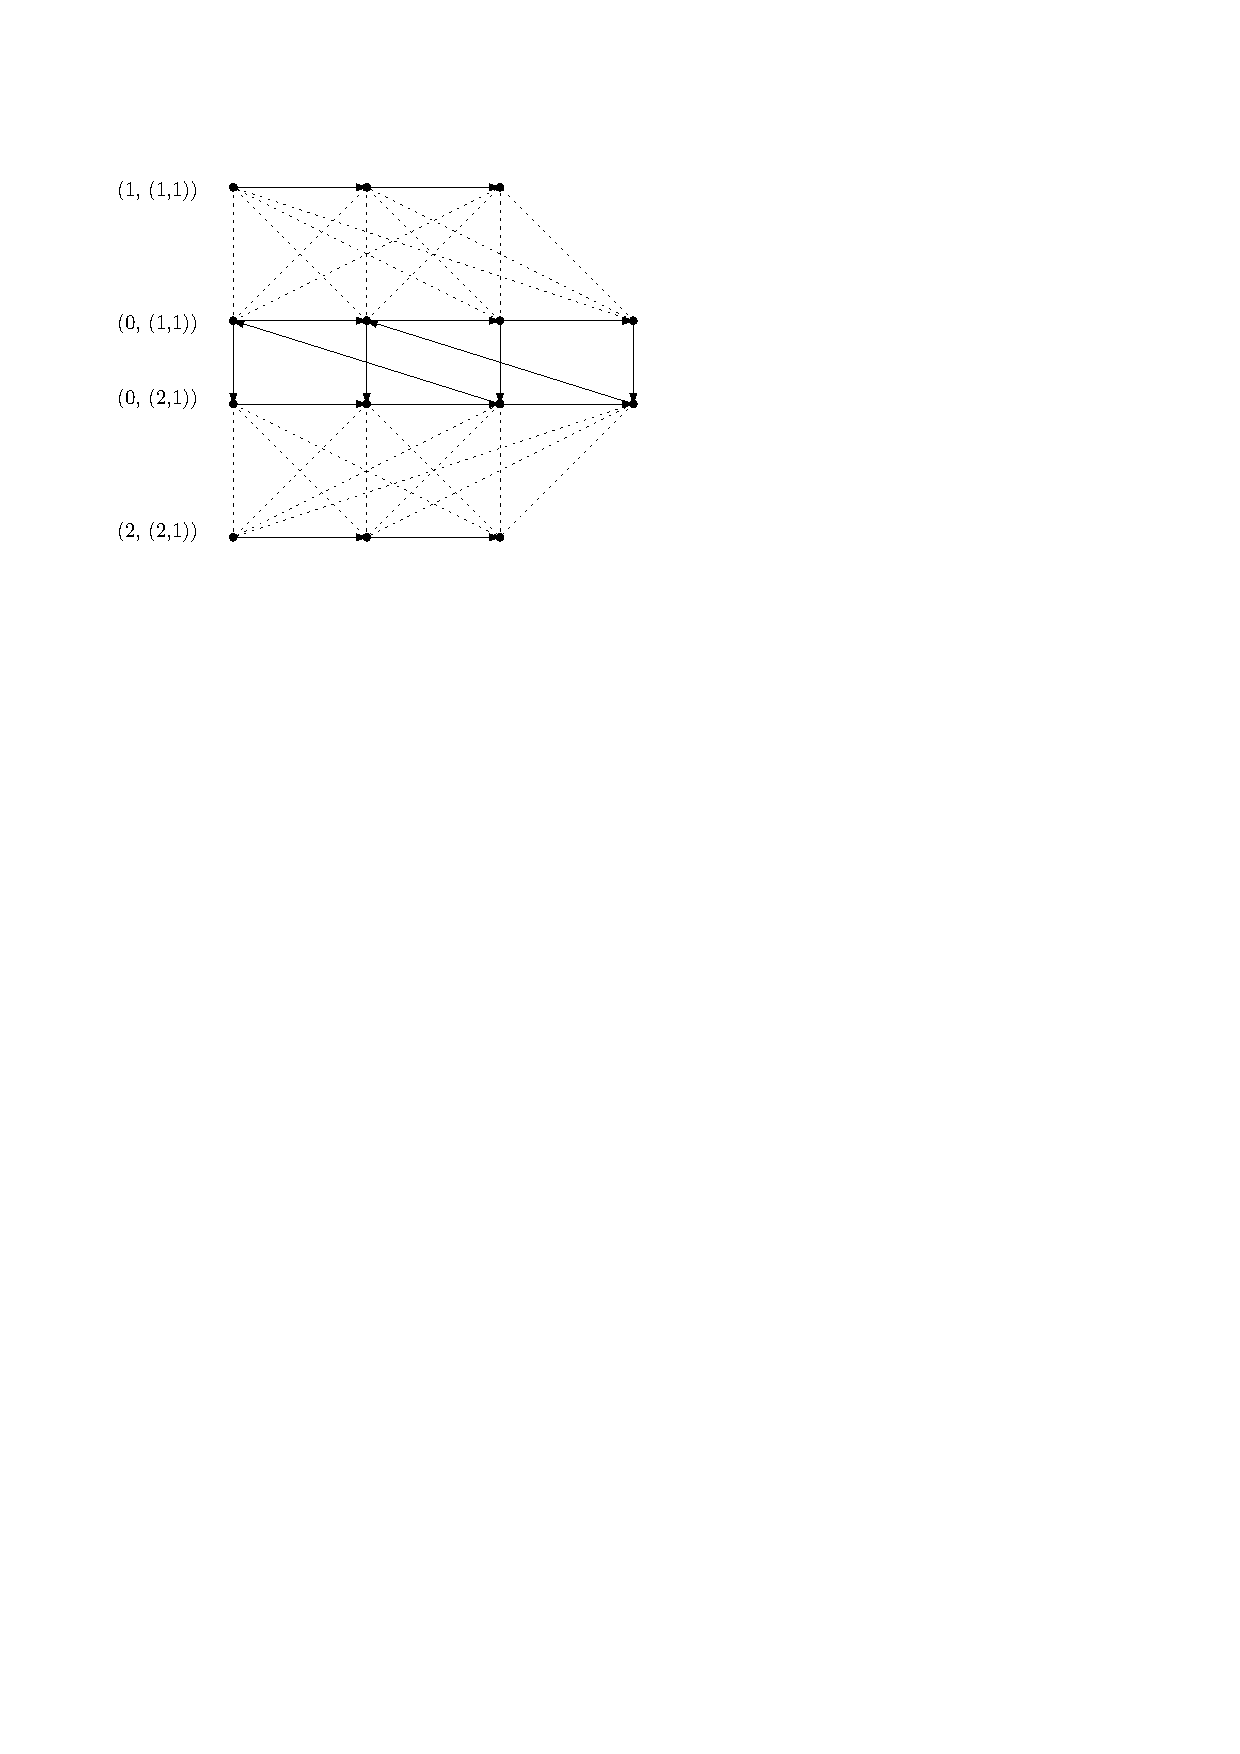
\includegraphics[scale=1]{figures/network/disjunctive_graph}
%  \caption{Empty disjunctive graph belonging to a tandem of two intersections,
%    labeled $v$ and $w$. There are three routes $\mathcal{R} = \{0, 1, 2\}$. On
%    route 0, four vehicle are arriving, the other two routes have 3 arrivals
%    each. Conjunctive arcs are drawn as from left to right, travel arcs are
%    drawn from top to bottom and disjunctive arcs are drawn as dotted lines. Two
%    buffer constraints are drawn as diagonal arcs, corresponding to a capacity
%    of 2 vehicles for the lane between both intersections.}
%  \label{fig:disjunctive_graph}
%\end{figure}

\newpage
\section{Learning to schedule}

Like in the single intersection case, we try to model optimal solutions using
autoregressive models.
%
In the single intersection case, we argued that each schedule is uniquely
defined by its route order $\eta$. Generalizing this to the case of multiple
intersections, we see that a schedule is uniquely defined by the set of route
orders $\eta^{v}$ at each intersection $v \in V$. Instead of working with such a set
of sequences, we will intertwine these sequences to obtain a single \textit{crossing sequence}
$\eta$, which consists of pairs $(r, v)$ of a route $r \in \mathcal{R}$ at some
intersection $v \in V_{r}$ and we will refer to such a pair as a \textit{crossing}. Of
course, this crossing sequence can be constructed in many different ways,
because it does not matter in which order the intersections are considered,
which is illustrated in Figure~\ref{fig:solution_equivalence}.
% \begin{align*}
%   | \{ t : \nu_{t} = v \} | = |\eta^{v}| \quad \text{ for each } v \in V ,
% \end{align*}
Given some problem instance $s$, we will consider autoregressive models of the form
\begin{align}
  \label{eq:autoregressive}
  p(\eta | s) =  \prod_{t=1}^{N} p(\eta_{t}| s, \eta_{1:t-1}) .
\end{align}

These models can also be understood in terms of a step-by-step schedule
construction process that transitions from a partial schedule state
$s_{t} = (s, \eta_{1:t})$ to the next state $s_{t+1}$ by selecting some \textit{action}
$\eta_{t+1} = (r_{t+1}, v_{t+1})$. We say a crossing is pending when it still has
unscheduled vehicles. Similarly, we say an intersection is pending when some of
its crossings are still pending. With these definitions, the set of \textit{valid actions}
$\mathcal{A}(s_{t})$ at some intermediate state $s_{t}$ is exactly the set of
pending crossings.
%
% multiple correct actions
We again emphasize that multiple sequences of actions lead to the same schedule,
because the order in which intersections are considered does not matter for the
final schedule, which is illustrated in Figure~\ref{fig:solution_equivalence}.
%
The models that we study can be understood as being parameterized as some
function of the disjunctive graph $G_{t}$ of partial schedule $s_{t}$, so an
alternative way of writing~\eqref{eq:autoregressive} that emphasizes this is
\begin{align}
  p(\eta = ((r_{1}, v_{1}), \dots, (r_{N}, v_{N})) \; | \; s) = \prod_{t=1}^{N} p(r_{t}, v_{t} | G_{t-1}) .
\end{align}
%
Instead of modeling the joint
probability distribution $p(r_{t}, v_{t} | G_{t-1})$ over crossings, we can also apply
the chain rule to factorize it as
\begin{align}
  p(r_{t}, v_{t} | G_{t-1}) = p(r_{t} | v_{t} , G_{t-1}) p (v_{t} | G_{t-1}) .
\end{align}
In this case, the model $p(r_{t} | v_{t}, G_{t-1})$ can be thought of as
predicting a set of actions, one for each intersection.

\begin{figure}
  \centering
  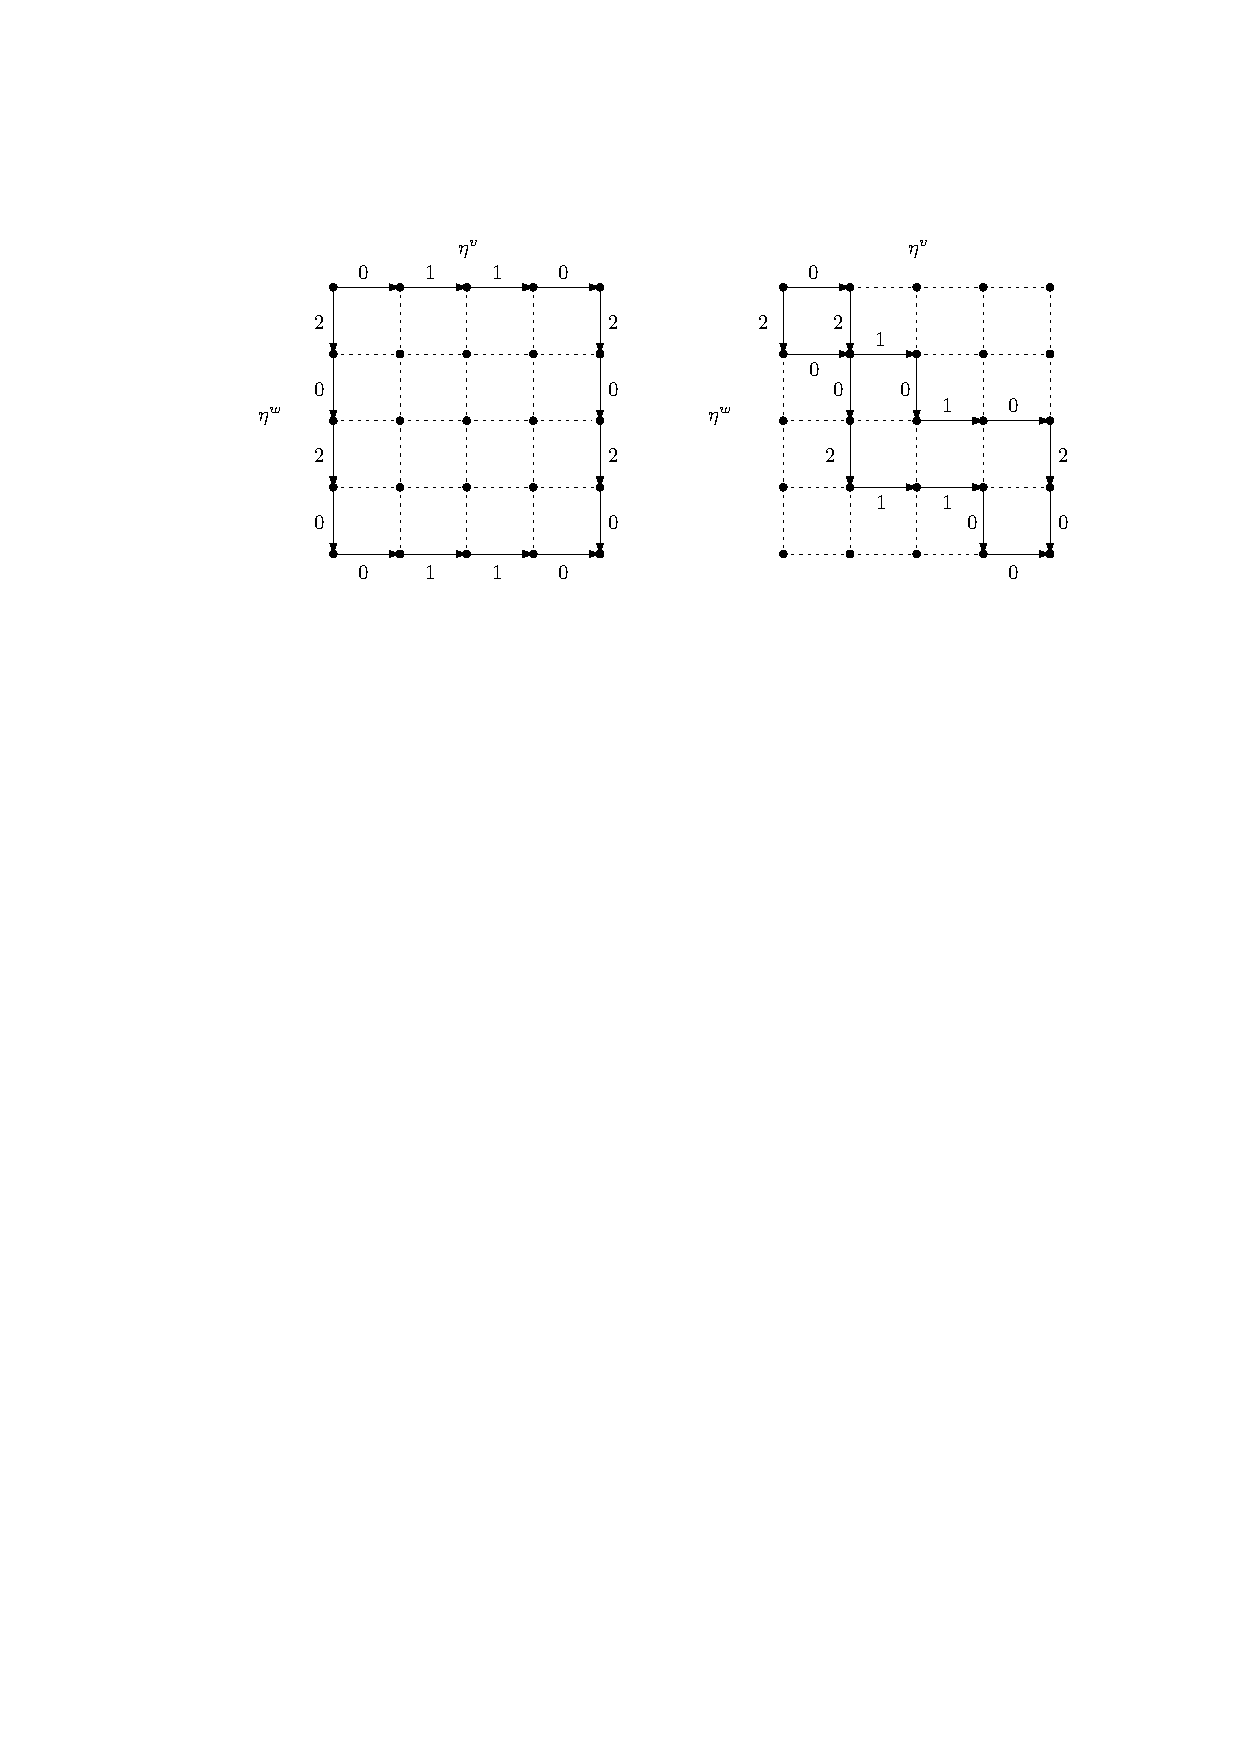
\includegraphics[width=0.9\textwidth]{figures/network/solution_equivalence}
  \caption{When each route order is locally fixed at every intersection, the
    global crossing sequence is not uniquely determined, because these local
    sequences may be merged in any order. Suppose we have a tandem of two
    intersections and a horizontal arrows correspond to taking the next local
    action at intersection $v$, a vertical arrows correspond to taking next
    local action at intersection $w$. Each valid crossing sequence corresponds
    to some path from the top-left to the bottom-right corner. Although any such
    crossing sequence produces the same schedule, it might be that our
    autoregressive model fits better on some sequences than others. For example,
    we might expect that sequences on the boundary of the grid, shown in the
    left grid, are harder to learn from data than sequences that stay closer to
    the diagonal, like in the right grid. The intuition is that we need to
    ``look into the future'' more to learn the former, while in the latter
    trajectories, progress in the two intersections is more balanced.}
  \label{fig:solution_equivalence}
\end{figure}

\paragraph{Intersection visit order.}
In the general class of autoregressive models for inputs and outputs with sets,
of which our model above is a special case (we have a set of sequences as
output), it has been noted before that the order in which inputs or outputs are
presented to the model during training has a considerable impact on the final
model fit~\cite{vinyalsOrderMattersSequence2016}.
%
For our model, we also expect to find this effect, so we will investigate the
impact of the order in which intersections are visited, determined by
$p(v_{t} | G_{t-1})$. We now propose some heuristic ways to define
$p(v_{t} | G_{t-1})$. Later, we will consider a neural network parameterization.
% random
First of all, the simple \textit{random} strategy would be to sample some
intersection with pending crossings at each step.
% ``boundary'' (or ``exhaustive'')
In the \textit{boundary} strategy, we keep visiting the same intersection until
it is done (when it has no pending crossings anymore), then move to some next
intersection. When the network of intersections is free of cycles, we could for
example follow some topological order. We use the term ``boundary'' because this
strategy produces trajectories along the boundary of the grid in
Figure~\ref{fig:solution_equivalence}.
% ``alternate''
In the \textit{alternating} strategy, we keep alternating between intersection to keep
the number of scheduled vehicles balanced among them. This produces trajectories
that can be understood as being close to the ``diagonal'' of the grid in
Figure~\ref{fig:solution_equivalence}. Again, the order in which we alternate between intersections may
again be based on some topological order.


\subsection{Model parameterization}

\subsubsection{Threshold heuristics}
It is straightforward to extend the threshold rule to networks of
intersections, when assuming a fixed intersection order. Each time some
next intersection is visited, we apply the single intersection threshold rule to
pick the next route. This is straightforward to do, because we can just consider
the disjunctive subgraph induced by the nodes belonging to that intersection to
arrive at the single intersection case.
%
Furthermore, the definition of the threshold rule itself does not depend on the
network of intersections. This is a desirable property, because it allows us to
tune the threshold on small networks and then apply it on larger ones.


\subsubsection{Neural constructive heuristic}
\label{sec:neural_constructive}

We will now propose a neural network parameterization of
$p(r_{t} | v_{t}, G_{t-1})$ and train it based on optimal schedules in a
supervised learning setting. The model can be best understood as solving a
so-called multi-label classification problem, because it needs to provide a
distribution over routes at every intersection.
%
The training data set $\mathcal{X}$ consists of pairs
$(G_{t-1}, (r_{t}, v_{t}))$, to which we refer to as \textit{state-action} pairs
to draw the parallel with the terminology used in the reinforcement learning
literature.
%
To obtain these pairs, we sample a collection of problem instances, which are
solved to optimality using a MILP solver. For each optimal schedule, we compute
the corresponding optimal route order $\eta^{v}$ for each intersection.
%
From these, we can construct $\mathcal{X}$ in different ways.
% sample a single intersection order for each instance
For example, for each solved instance, we can randomly select some intersection
order $\mu$, which fixes the crossing order $\eta$. We can then replay
this sequence of actions step-by-step to obtain the corresponding sequence of
state-action pairs.
% multiple intersection order per instance
The model might become more robust when training on multiple samples of
intersections orders per instance.
% fixed intersection order
Alternatively, we can consider one of the fixed intersection orders
described at the start of this section (random, boundary, alternating).
% lookahead
Furthermore, combined with one of the above strategies, we can also employ some
kind of fixed lookahead procedure, as illustrated in
Figure~\ref{fig:state_action_collection}.
% inference
At inference time, we use the same intersection order as during training and at
each step we greedily select $r_{t}$.

%\begin{figure}
%  \centering
%  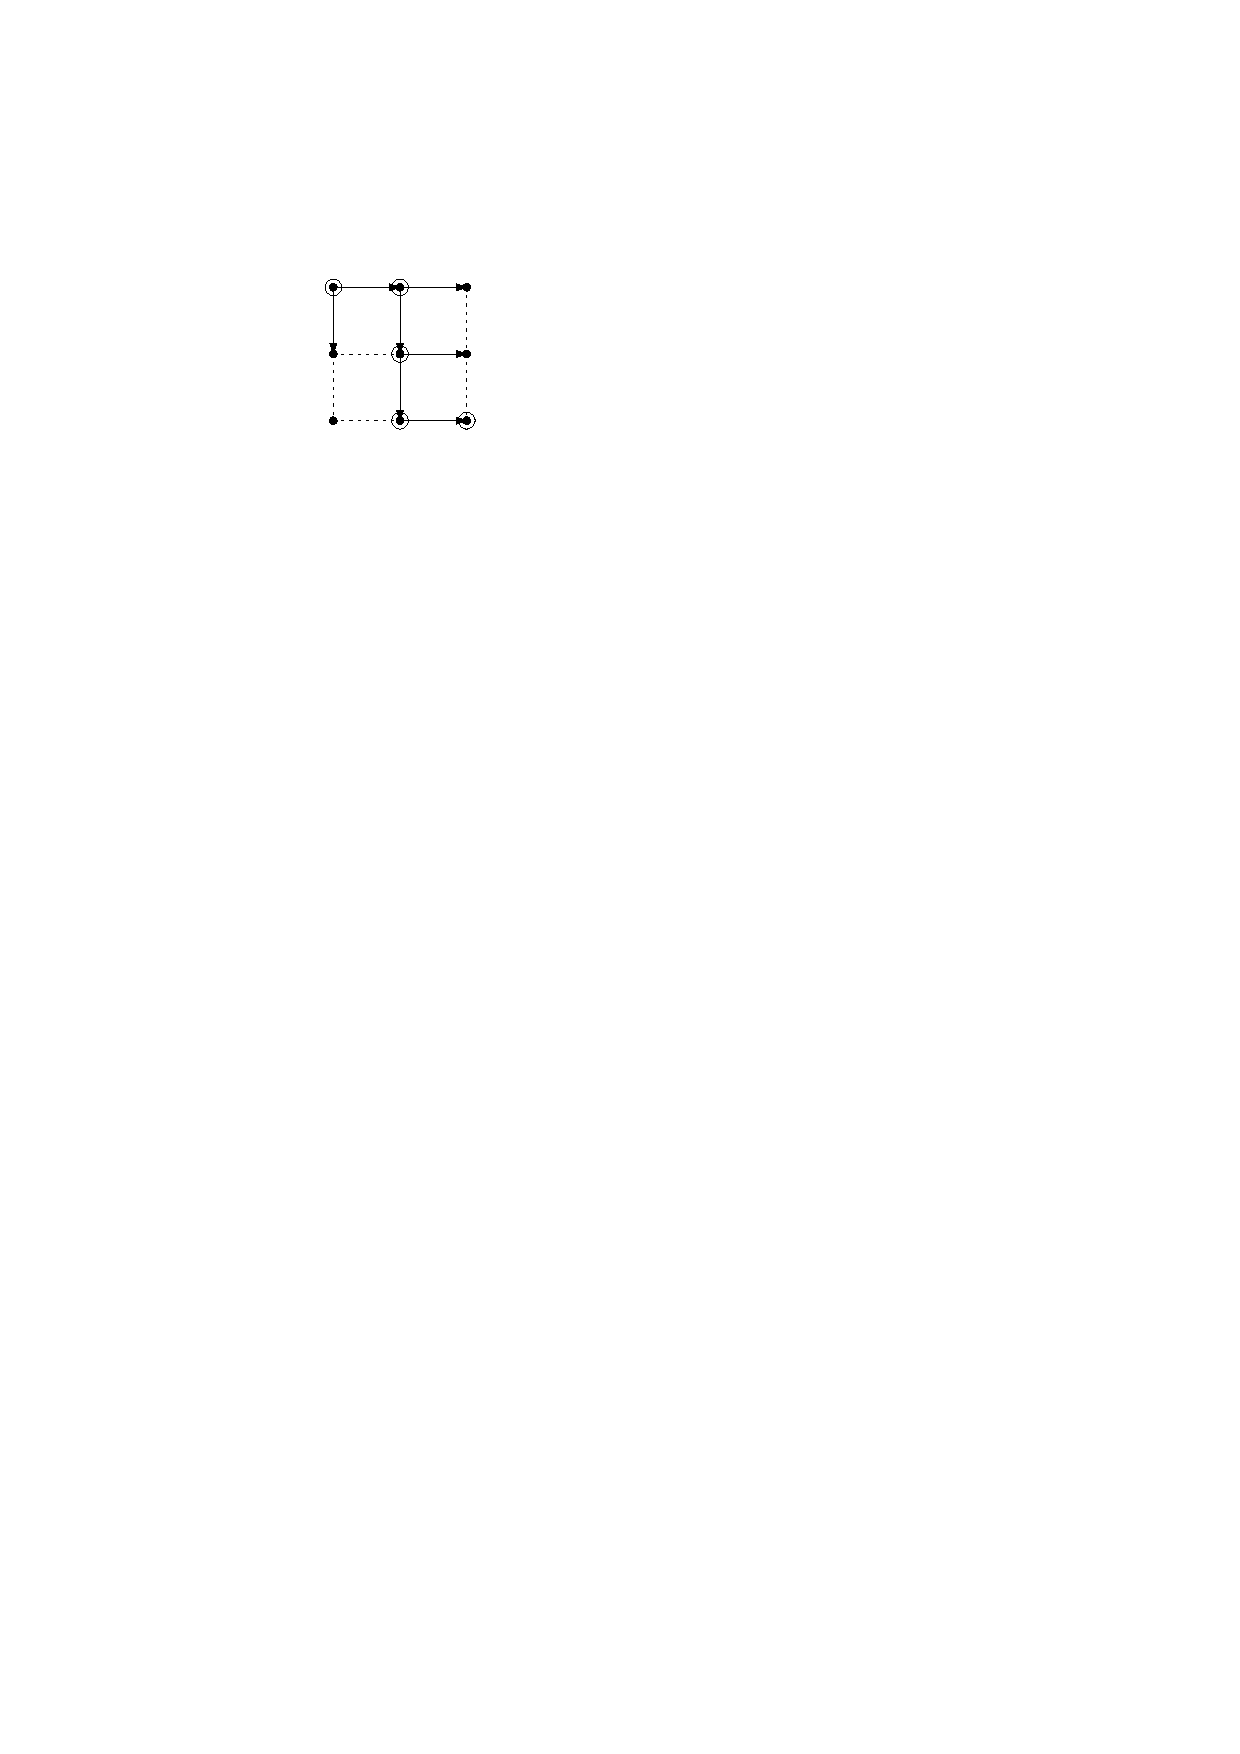
\includegraphics[scale=1.2]{figures/network/state_action_collection}
%  \caption{Possible strategy for collecting state-action pairs: one action
%    look-ahead. At every state $s_{t}$ with a set of possible actions
%    $\mathcal{A}(s_{t})$, we add all state-action pairs
%    $\{ (s, a) : a \in \mathcal{A}(s) \}$, but we pick a single action $a^{*}$
%    to move to the next state. In the figure, the state-action pairs are
%    depicted as solid arrows. The encircled dots are the states that are
%    actually visited. Observe that this procedure can be naturally generalized
%    to a look-ahead of arbitrary depth.}
%  \label{fig:state_action_collection}
%\end{figure}

We will now describe how the model is parameterized based on recurrent
embeddings of the sequences of crossing time lower bounds at each crossing, in a
somewhat similarly to how we used the horizons in the single intersection model.
%
Let $k(r, v)$ denote the number of scheduled vehicles at crossing $(r, v)$ and
let $n_{r}$ denote the total number of vehicles on route $r$. For each crossing
$(r, v)$, consider the earliest crossing time of the next unscheduled vehicle,
which we denote as
\begin{align*}
  T(r, v) = \beta(r, k(r, v) + 1, v) .
\end{align*}
We define the \textit{horizon} of crossing $(r, v)$ to be the sequence of relative lower bounds
\begin{align*}
  h(r, v) = (\beta(r, k(r, v) + 2, v) - T, \dots, \beta(r, n_{r}, v) - T) .
\end{align*}
%
Each such horizon is embedded using an Elman RNN. To produce a logit for each
crossing, these embeddings are fed through a feedforward network, consisting of
two hidden layers of size 128 and 64 neurons with relu activation and batch
normalization layers in between. See Figure~\ref{fig:rnn_model} for a schematic
overview of the architecture. {\color{Navy} Next: instead of $h(r, v)$, feed
  $(T(r, v), h(r, v))$ to the FF.}

%\begin{figure}
%  \centering
%  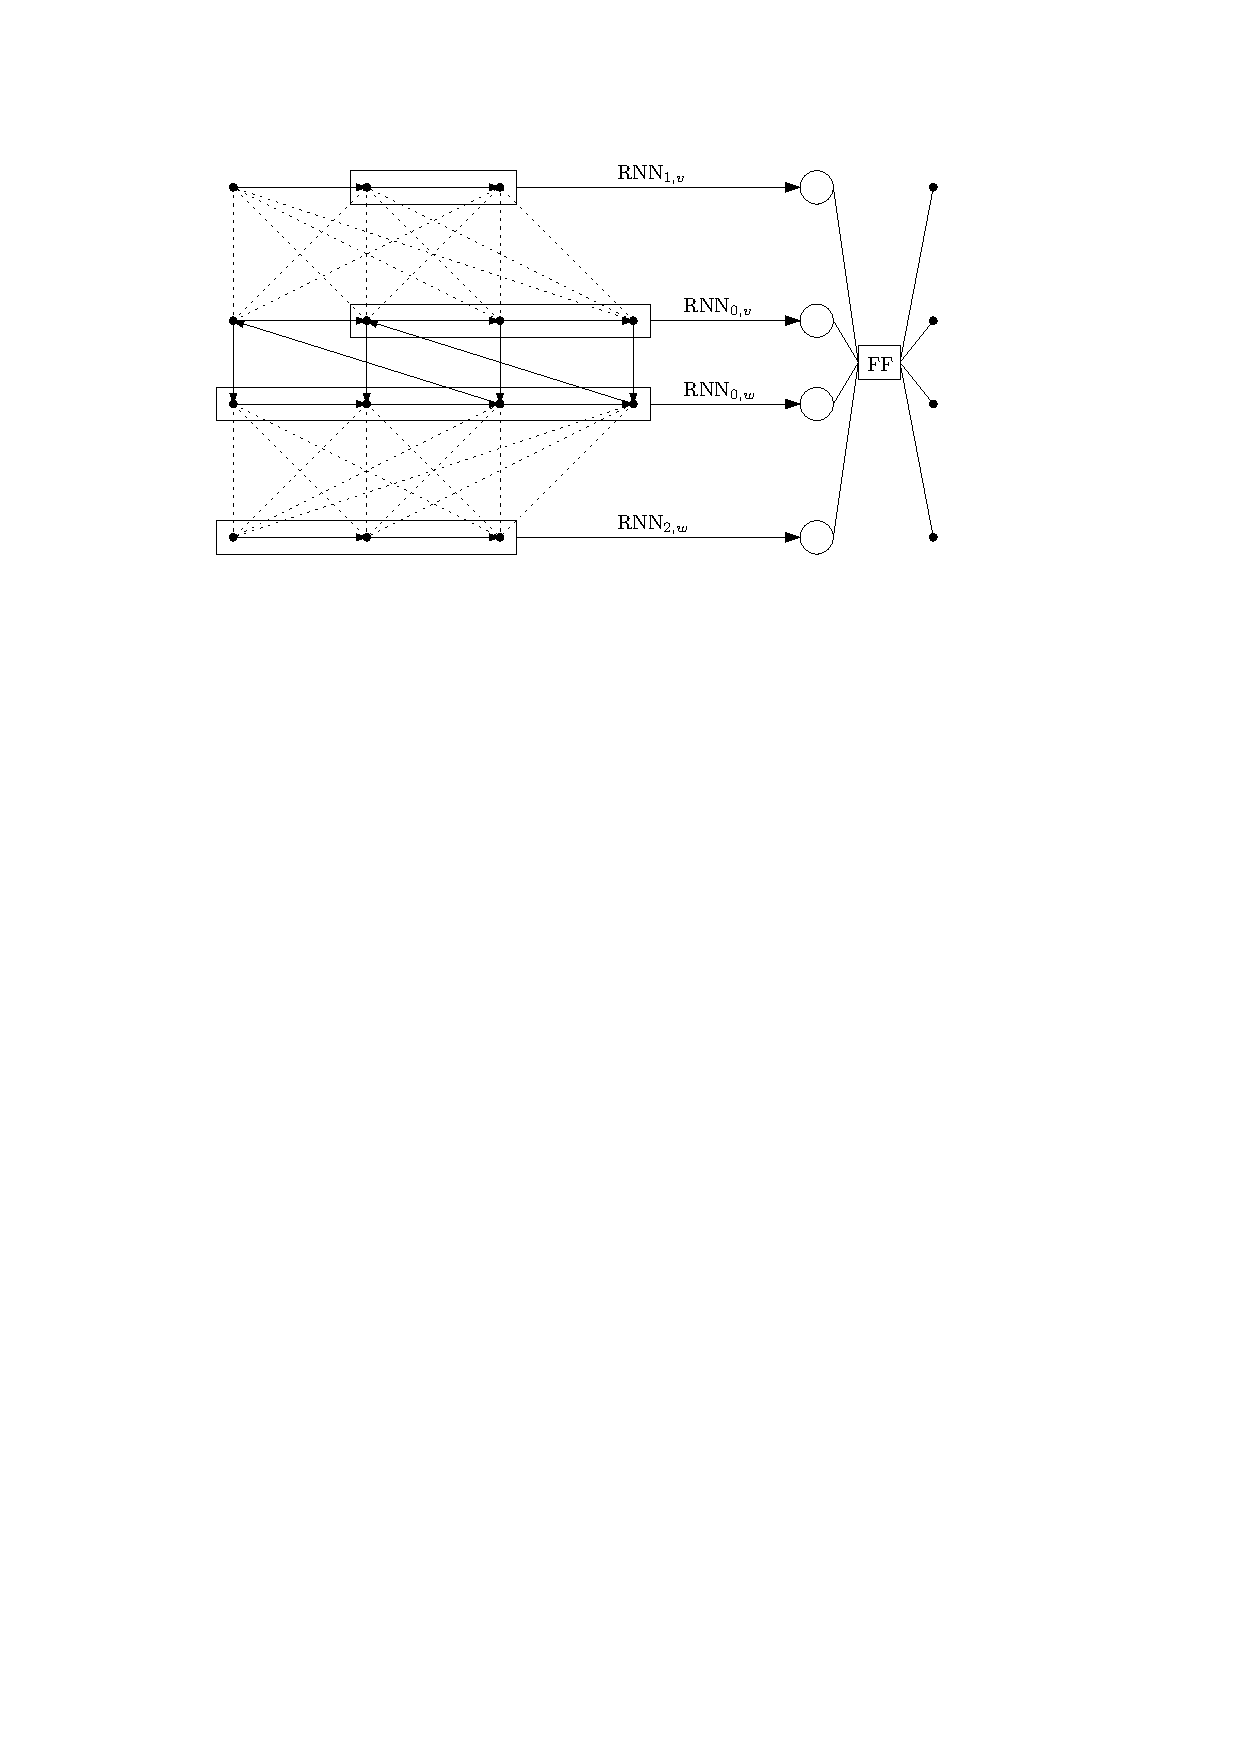
\includegraphics[scale=1]{figures/network/rnn_model}
%  \caption{Illustration of model with RNN encoding of horizon at each crossing.
%    The disjunctive graph nodes whose lower bounds are part of the current
%    horizons are indicated with rectangles. The RNN embeddings (open circles)
%    are fed through a final feedforward network to produce a logit (dots) for
%    each crossing.}
%  \label{fig:rnn_model}
%\end{figure}

To train the model, we use the Adam optimizer with learning rate~$10^{-4}$ and a
batch size of $40$ state-action pairs. We experienced a case of the exploding
gradients problem when we did not use the batch normalization layers. To allow a fair comparison of methods accross instances of different
sizes, both in terms of the number of vehicles and the size of the network, we
adapt both objective as follows.
% objective variant 1
For the first variant, we divide by the total number of vehicles, so we report
$\text{obj}_{1}(y) / |\mathcal{N}|$. Given some problem instance, let $N$ denote
the length of a crossing sequence, so it is also the total number of
vehicle-intersection pairs $(i, v)$ that need to be scheduled. For the second
objective variant, we consider the average delay per vehicle-intersection pair,
so we report $\text{obj}_{2}(y) / N$, which we report in Table~\ref{tab:results}.

% silent package loading


\begin{knitrout}
\definecolor{shadecolor}{rgb}{0.969, 0.969, 0.969}\color{fgcolor}\begin{table}
\centering
\caption{\label{tab:results}Average scaled optimal objective value computed using MILP and using the threshold heuristic with threshold $\tau = 0$. Each class of problem instances is identified by the number $n$ of vehicle arrivals per route and the grid network size as cols x rows.}
\centering
\resizebox{\ifdim\width>\linewidth\linewidth\else\width\fi}{!}{
\begin{tabular}[t]{cc|cc|c|c|c|ccc|cc|c|c|c|ccc|cc|c|c|c|ccc|cc|c|c|c|ccc|cc|c|c|c|ccc|cc|c|c|c|ccc|cc|c|c|c|ccc|cc|c|c|c|c}
\toprule
n & size & MILP & time & $\tau = 0$  (gap) & random (gap) & boundary (gap) & alternate (gap)\\
\midrule
5 & 2x1 & 57.27 & 0.06 & 65.27 (11.45\%) & 58.96 (2.95\%) & 58.72 (2.52\%) & 58.23 (1.66\%)\\
5 & 3x1 & 57.67 & 0.12 & 68.34 (15.44\%) & 59.77 (3.65\%) & 59.82 (3.74\%) & 58.72 (1.83\%)\\
5 & 3x2 & 57.35 & 1.38 & 69.17 (18.32\%) & 60.88 (6.16\%) & 60.36 (5.25\%) & 58.82 (2.56\%)\\
\bottomrule
\end{tabular}}
\end{table}

\end{knitrout}



\subsection{Reinforcement learning}

Instead of using a fixed training set $\mathcal{X}$ of state-action pairs during
training, we can fit our model from the perspective of a reinforcement learning
problem, which we already alluded to in Section~\ref{sec:neural_constructive}.
%
More precisely, given some scheduling problem instance $s$, we are dealing with
a Deterministic Markov Decision Process (DMDP), where partial disjunctive graphs
serve as states and crossings correspond to actions.
%
The potential benefit of using reinforcement learning is that we do not have to
fix an intersection order: our hope is that the training procedure will
automatically converge to some good intersection order.

{\color{Navy} The threshold heuristic ($\tau = 0$) can provide a
  \textit{baseline} for reinforcement learning, reducing the variance of the
  REINFORCE estimator.}

{\color{Navy} N.B. The step-numbering is different in
  $G_{0},\eta_{1},G_{1},\eta_{2}, \dots$ from the common RL notation
  $S_{0},A_{0},R_{1},S_{1},A_{1},\dots$, so generally $A_{t} = \eta_{t+1}$.}


\bibliography{references}
\bibliographystyle{ieeetr}


\end{document}

% to enable the minted package
% Local Variables:
% TeX-command-extra-options: "-shell-escape"
% End:
